% ---------------------------------------------------------------------------
% Author guideline and sample document for EG publication using LaTeX2e input
% D.Fellner, v1.13, April 29, 2009

\documentclass{egpubl}
\usepackage{sca2012}

% --- for  Annual CONFERENCE
% \ConferenceSubmission % uncomment for Conference submission
% \ConferencePaper      % uncomment for (final) Conference Paper
% \STAR                 % uncomment for STAR contribution
% \Tutorial             % uncomment for Tutorial contribution
% \ShortPresentation    % uncomment for (final) Short Conference Presentation
%
% --- for  CGF Journal
% \JournalSubmission    % uncomment for submission to Computer Graphics Forum
% \JournalPaper         % uncomment for final version of Journal Paper
%
% --- for  EG Workshop Proceedings
\WsSubmission    % uncomment for submission to EG Workshop
% \WsPaper         % uncomment for final version of EG Workshop contribution
%
 \electronicVersion % can be used both for the printed and electronic version

% !! *please* don't change anything above
% !! unless you REALLY know what you are doing
% ------------------------------------------------------------------------

% for including postscript figures
% mind: package option 'draft' will replace PS figure by a filname within a frame
\ifpdf \usepackage[pdftex]{graphicx} \pdfcompresslevel=9
\else \usepackage[dvips]{graphicx} \fi

\PrintedOrElectronic

% prepare for electronic version of your document
\usepackage{t1enc,dfadobe}

\usepackage{egweblnk}
\usepackage{cite}

% For backwards compatibility to old LaTeX type font selection.
% Uncomment if your document adheres to LaTeX2e recommendations.
% \let\rm=\rmfamily    \let\sf=\sffamily    \let\tt=\ttfamily
% \let\it=\itshape     \let\sl=\slshape     \let\sc=\scshape
% \let\bf=\bfseries

% end of prologue

% ---------------------------------------------------------------------
% EG author guidelines plus sample file for EG publication using LaTeX2e input
% D.Fellner, v1.17, Sep 23, 2010


\title[ A Hybrid Method for Adaptive SPH Fluid Simulation ]%
      { A Hybrid Method for Adaptive SPH Fluid Simulation }

% for anonymous conference submission please enter your SUBMISSION ID
% instead of the author's name (and leave the affiliation blank) !!
\author[1158]
       {1158
%        S. Spencer$^2$\thanks{Chairman Siggraph Publications Board}
        \\
% For Computer Graphics Forum: Please use the abbreviation of your first name.
%         Stony Brook University, USA
%        $^2$ Another Department to illustrate the use in papers from authors
%             with different affiliations
       }

% ------------------------------------------------------------------------

% if the Editors-in-Chief have given you the data, you may uncomment
% the following five lines and insert it here
%
% \volume{27}   % the volume in which the issue will be published;
% \issue{1}     % the issue number of the publication
% \pStartPage{1}      % set starting page


%-------------------------------------------------------------------------
\begin{document}

 \teaser{
  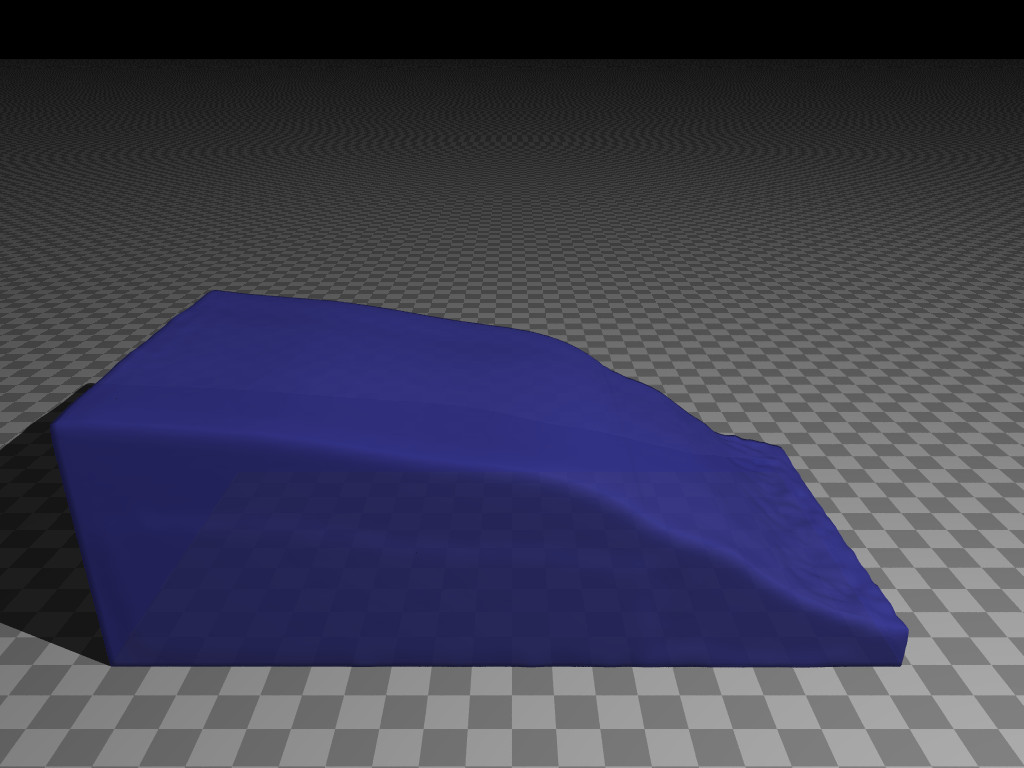
\includegraphics[width=.3\linewidth]{title-1}
  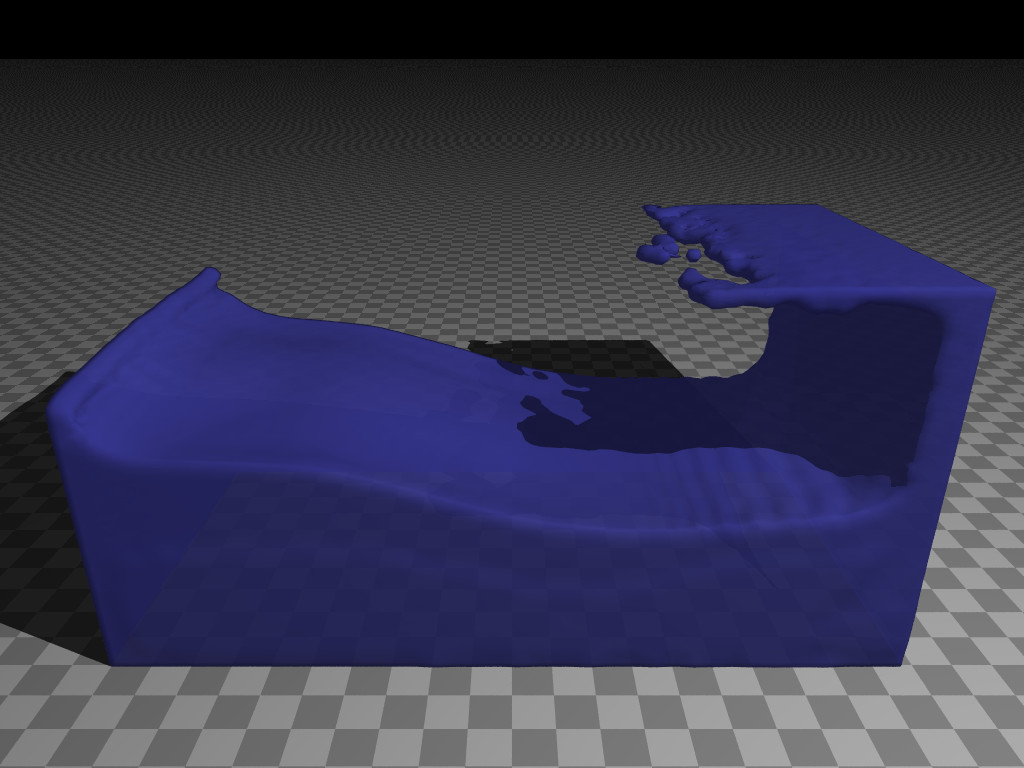
\includegraphics[width=.3\linewidth]{title-2}
  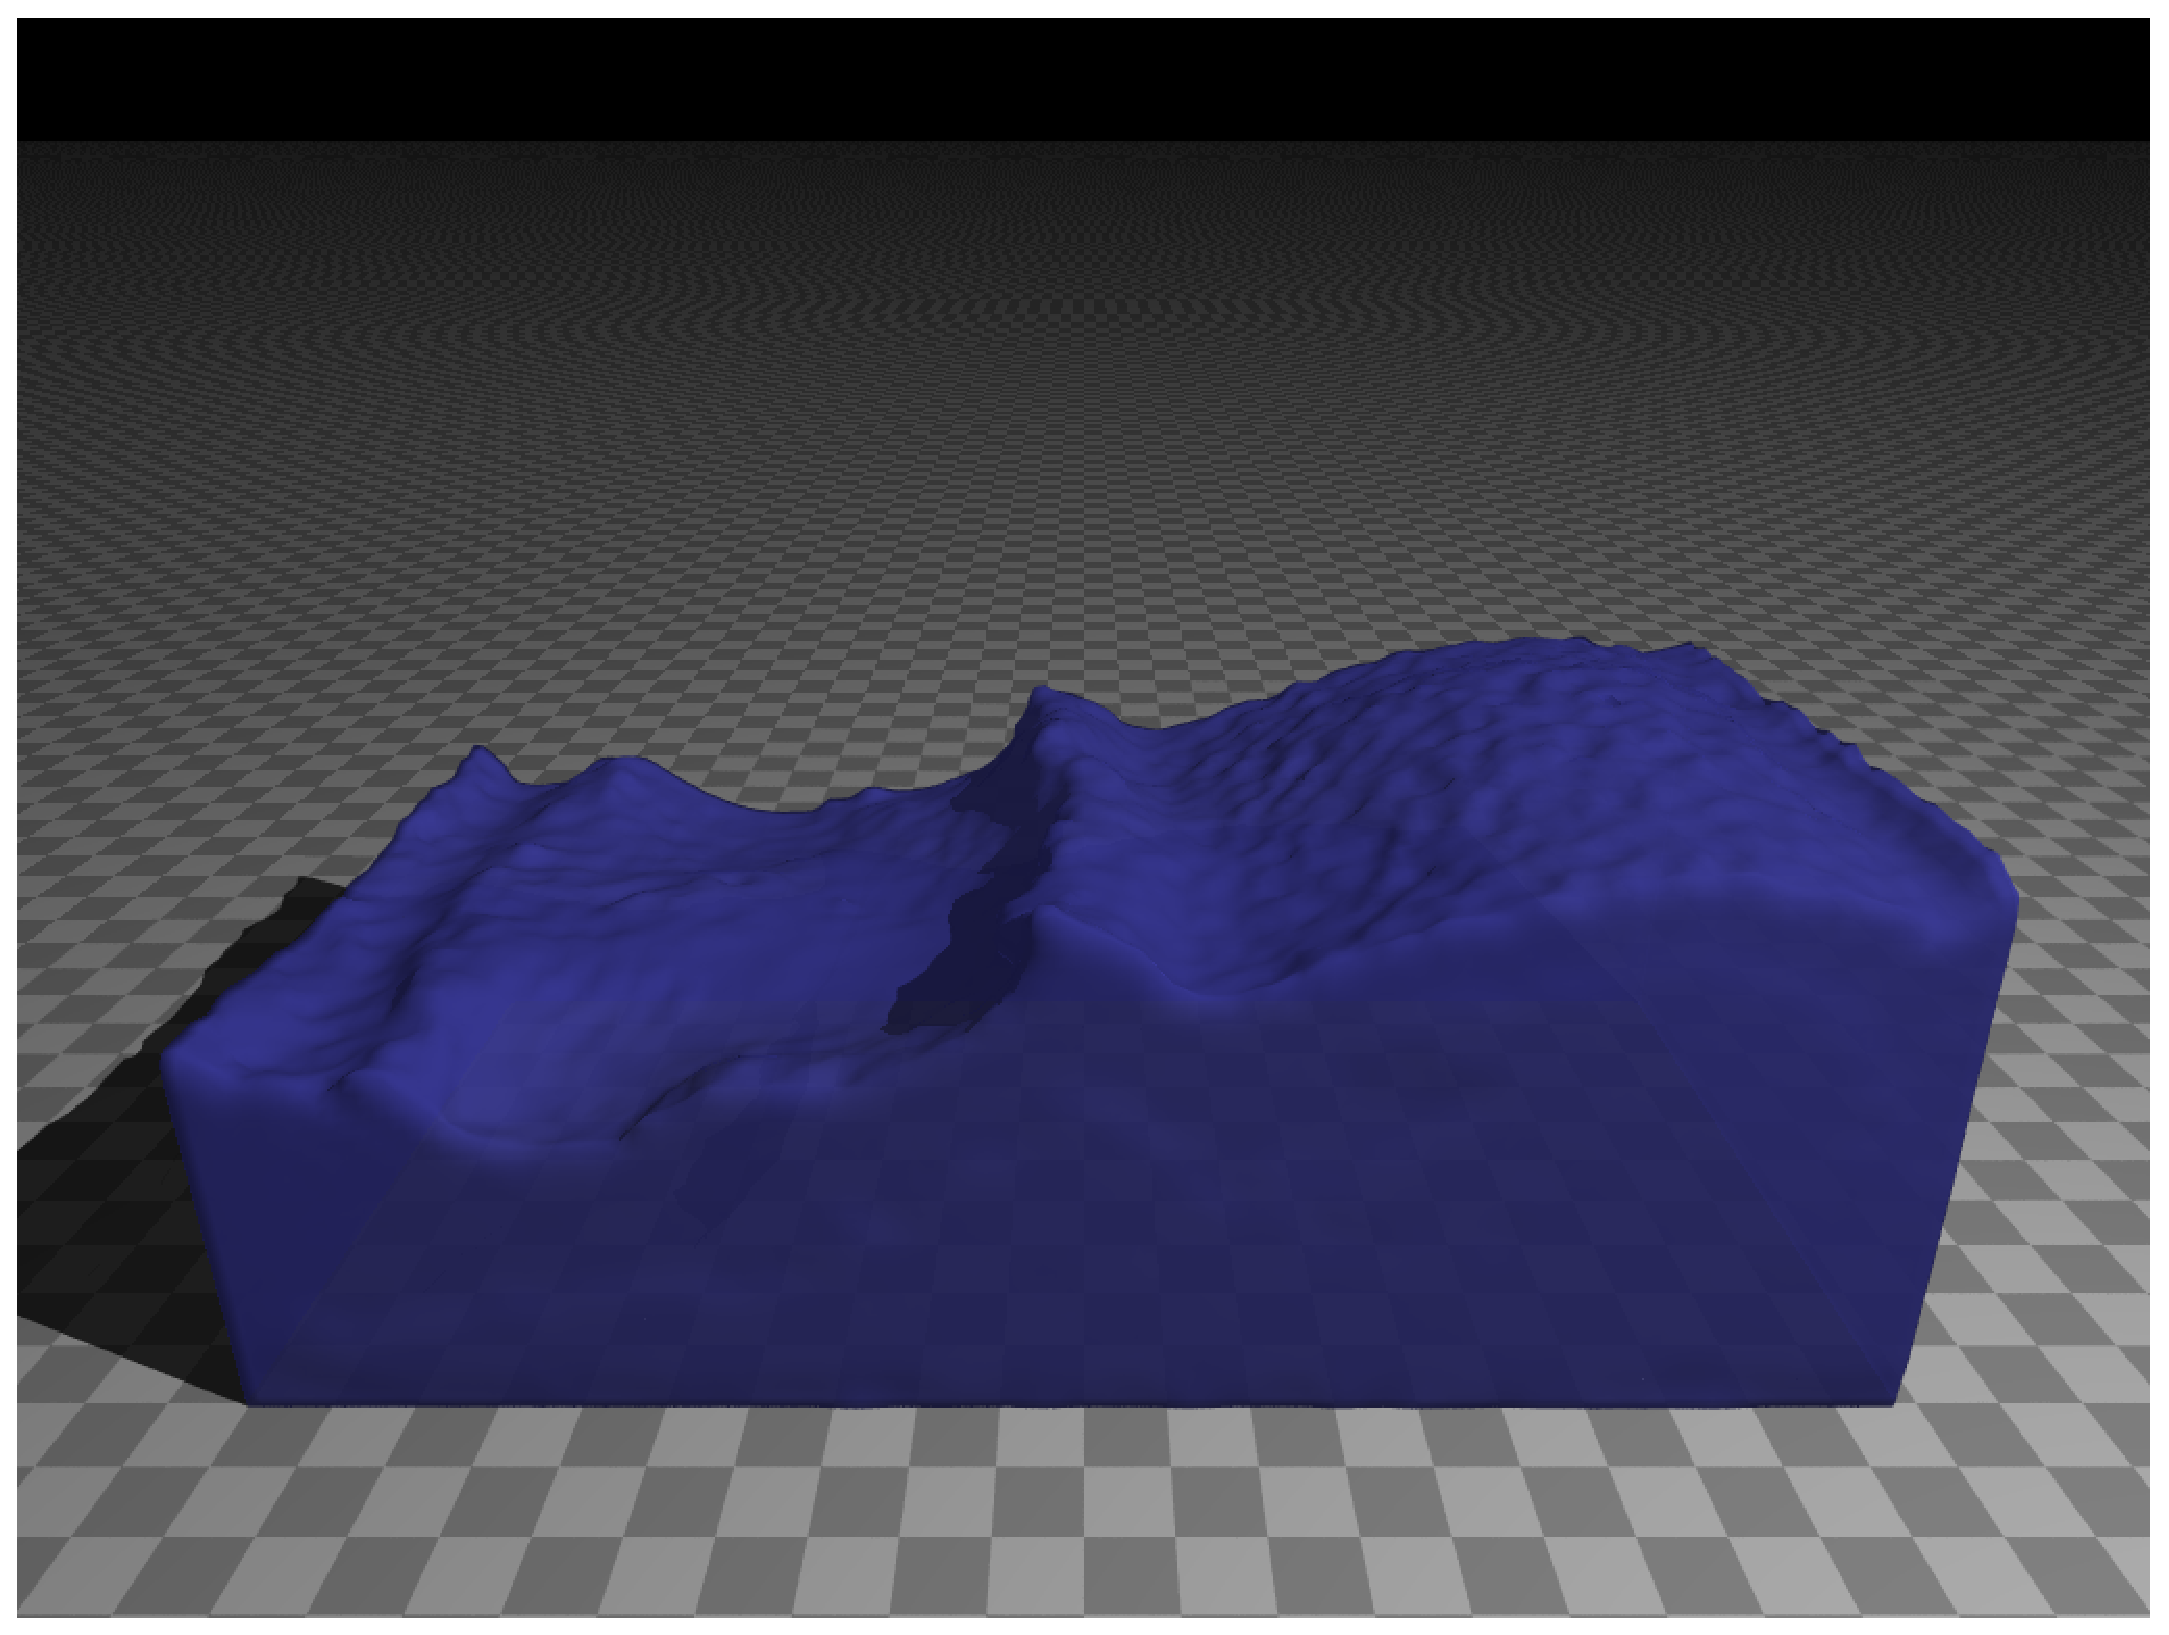
\includegraphics[width=.3\linewidth]{title-3}
  \centering
   \caption{Fluid simulation with our approach.}
 \label{fig:teaser}
 }

\maketitle

\begin{abstract}

  This paper proposes a new hybrid approach to adaptive SPH fluid
  simulation that better handles particle splitting and merging.
  Simulation of SPH fluid with adaptive, multiple-sized particles
  could enhance the animation performance while still retaining
  dynamic details with high-fidelity visual effects. However,
  conventional algorithms primarily refine simulation near fluid
  surface or in highly deformable region in spatial domain. We
  advocate a novel criterion that is based on the hybrid of both
  physics and geometry, and it is operated in both space domain and
  frequency domain. In particular, we use distance field as geometry
  criterion to localize region near fluid surface and we use
  wavelet-transformed energy in frequency domain as physics criterion
  to accurately detect inter-fluid turbulent region. Our adaptive SPH
  method based on space and frequency domain analysis is more accurate
  compared to the previous approaches. By coupling physics and
  geometry together, we could effectively detect regions that require
  particle splitting or merging. Moreover, our hybrid method is
  especially necessary to detect inner-fluid turbulent region and
  identify fine-detailed interface between different materials
  anywhere within fluid. We also propose a new surface tension model
  by integrating the air resistance into simulation, making the
  simulation more physically accurate. Through various animation
  scenarios, we demonstrate the efficacy and effectiveness of our new
  approach for high-fidelity fluid simulation.

\begin{classification} % according to http://www.acm.org/class/1998/
\CCScat{Computer Graphics}{I.3.7}{Computer Graphics}{Three-Dimensional Graphics and Realism}
\end{classification}

\end{abstract}

%-------------------------------------------------------------------------
\section{Introduction}

Fluid simulation necessarily requires very high matter discretization
and spatial resolution to preserve dynamic and surface details and to
generate appealing visual effects for graphics applications. Towards
these goals, a high resolution grid is required in Eulerian grid
method, and a very large number of particles are demanded in Smoothed
Particle Hydrodynamics (SPH) method. Therefore, it is much more
desirable to only allocate computing resources to regions where
complex flow behavior emerges. With the help of octree data structure,
\cite{Losasso:2004:SWS:1015706.1015745} generates highly realistic
water behavior, by adaptively solving the full three-dimensional
Navier-Stokes equations in a grid-based system.

There are also some works addressing this problem in Lagrangian
method, for example, the SPH method. By dynamically and adaptively
splitting large particles into small particles and merging small
particles into large ones, we could use large particles to simulate
the gross shape of fluid but small particles to animate turbulent
features (e.g., splash, vortex) and surface details (e.g., wave). We
could sample the turbulent areas according to geometry
\cite{Adams:2007:ASP:1276377.1276437}, physics
\cite{Hong:2008:API:1394332.1394340} or both
\cite{Yan:2009:RFS:1568678.1568695}.

In this paper, we propose a new criterion governing particle splitting
and merging. Our method is both physically and geometrically based. It
may be noted that, \cite{Hong:2008:API:1394332.1394340} is also based
on physics. In \cite{Hong:2008:API:1394332.1394340}, Hong et al. used
the concept of Reynolds number as part of criterion. But this Reynolds
number is only computed in spatial domain. Reynolds number is the
value sampled at isolated points. It contains no information about its
neighboring region. In our method, we use the wavelet-transformed
energy as criterion. Wavelet analysis is an efficient and accurate
mathematical tool to analyze data at different scales. In both
\cite{Kim:2008:WTF:1360612.1360649} and \cite{PG2011short:67-72:2011},
the wavelet-inspired technique is used as a tool to detect and
compensate energy lost in order to preserve details. To the best of
our knowledge, the work proposed in this paper is the first attempt to
utilize wavelet analysis as a tool to help guide particle splitting
and merging. Since this analysis is in frequency domain, we have a
more global knowledge about the overall energy distribution.

Since the merging and splitting of particles at different level of
scales may overburden any desktop animation system by introducing
heavy computational cost, we simulate the fluid with particles in only
two scales in this paper. Therefore, attributes including kernel
length and particle mass are fixed values for particles in each layer.
This way, we could precompute and cache them in the interest of time
performance.

Our method has the following contributions:

\begin{itemize}

\item We propose a new adaptive SPH fluid simulation algorithm based
  on the hybrid of physics and geometry. When guiding SPH particle
  splitting and merging, we conduct rigorous analysis in both space
  and frequency domains. This is the first attempt to use wavelet
  analysis to guide particle splitting and merging in adaptive SPH
  fluid simulation. Our method is founded upon a solid foundation in
  both mathematics and physics.

\item We also propose a new surface tension model by integrating the
  air resistance into simulation, making the simulation more
  physically accurate. We integrate the air into our simulation by
  applying the air resistance. Traditional SPH fluid simulations do
  not consider the interaction between fluid surface and air. In
  \cite{Schechter:2012:GSA:2185520.2185557}, air particles are
  periodically sampled near the fluid surface. But this sampling
  process is complex. By involving the air resistance, we could
  approximate the interaction between fluid and air while avoiding the
  complex particle sampling process.

\end{itemize}

%-------------------------------------------------------------------------
\section{Related Works}

In this section, we shall briefly review the previous works relevant
to the central theme of this paper. Since our method is a particle
based method, we should primarily concentrate on the discussion of the
particle based methods that have been developed previously.

Generally speaking, there are two physically based ways to simulate
fluids, Eulerian method and Lagrangian method. They are all based on
the Navier-Stokes equation. Eulerian method solves the Navier-Stokes
equation over a grid tessellation. \cite{Foster:1996:RAL:244304.244315}
is perhaps the first to apply the Navier-Stokes equation to 3D liquid
simulation in computer graphics field for incompressible fluid. But
this algorithm is not stable enough. Later on,
\cite{Stam:1999:SF:311535.311548} designs an algorithm to guarantee
the stability of fluid simulation by utilizing a semi-Lagrangian
scheme to handle velocity advection. This algorithm is always stable
for arbitrary time steps. Because of the computational cost of
Eulerian method, it is hard to simulate fluid with a fine grid in
real-time.  \cite{Chentanez:2011:REW:2010324.1964977} proposes a new
Eulerian fluid simulation method in real-time by utilizing a hybrid
grid representation consisting of regular cubic cells on top of a
layer of tall cells.

Because of the numerical dissipation introduced in the Eulerian
method, the particle based Lagrangian methods play a more and more
important role in recent research and the most promising approach
among them is arguably the SPH method.
\cite{Muller:2003:PFS:846276.846298} is the first to introduce the SPH
method to the simulation of water. Later on, the SPH method is
extended to the simulation of interaction between different fluids
\cite{Muller:2005:PFI:1073368.1073402} and animation of viscoelastic
fluid \cite{Clavet:2005:PVF:1073368.1073400}.  There is also research
about parallel implementation of SPH algorithm
\cite{Harada_Koshizuka_Kawaguchi_2007}.

Besides fluids, people also simulate smoke by the combination of
particle system and grid system method, like FLIP
\cite{Zhu:2005:ASF:1073204.1073298}. By generating some vortex
particles in the grid and coupling the particles with grid based on
vorticity confinement, \cite{Selle:2005:VPM:1073204.1073282} can
improve the turbulent effects for water, smoke, and explosion.
\cite{CGF:CGF1562} can simulate multiple speed smoke by simulating the
low speed smoke in grid and high speed smoke in particle system.
\cite{Cohen:2010:IFS:1730804.1730807} proposes an interactive system
featuring fluid-driven animation that could respond to moving objects.
It would generate a grid coupled with the moving object and simulate
the smoke near the object in the grid system. For particles moving out
of the surrounding grid, the smoke would be animated in a pure
particle system.

%%%obscuring the point at which the fluid simulation
%%%ends.

Because the energy driven approach is always strictly physics based in
computer graphics, energy based fluid and smoke simulation is also an
active research topic. We could compensate the energy lost back to the
simulation system in order to preserve the details.
\cite{Kim:2008:WTF:1360612.1360649} analyzes the wavelet-transformed
energy in the low resolution grid system in frequency domain and then
synthesizes the wavelet turbulence energy to the high resolution grid
to preserve turbulence features. Instead of the grid system,
\cite{PG2011short:67-72:2011} applies the algorithm in
\cite{Kim:2008:WTF:1360612.1360649} to the particle system to conserve
the wavelet turbulence energy in SPH. In
\cite{Kim:2008:WTF:1360612.1360649}, we do not need to transfer the
particle attribute to the auxiliary grid but directly work in the
point cloud. Instead of isotropic noise,
\cite{Pfaff:2010:SFS:1882261.1866196} adds the procedural approach
based turbulence by generating and advecting turbulence particles
based on anisotropic noise. Simulation based on anisotropic noise
could make a more appealing visual effect than simulation based on
isotropic noise alone.

In a particle system, the computing efficiency could be improved by
constructing the particle system adaptively. It can make the
distribution of computing resources more reasonable and reduce the
complexity of calculation. For regions that do not need to preserve
details, fewer particles would be enough; while for physically and
visually important regions, a larger number of particles are required
instead. \cite{Desbrun:1996:SPN:274976.274981} first applies the
adaptive particle system to the simulation of highly deformable
models. \cite{Adams:2007:ASP:1276377.1276437} analyzes the particle
system based on the extended local feature size to decide when to
split or merge particles. This concept of extended local feature size
is purely geometry based, but the turbulent regions computed with this
method obey the rules in physics. Unlike
\cite{Adams:2007:ASP:1276377.1276437}, which simulates compressible
fluid, \cite{Hong:2008:API:1394332.1394340} can simulate
incompressible fluid by the application of the FLIP
\cite{Zhu:2005:ASF:1073204.1073298} algorithm. This method computes
the advection with SPH but analyzes the deformability of fluid and
conserves incompressibility by transferring the particle attribute
value to the auxiliary grid system.
\cite{Yan:2009:RFS:1568678.1568695} samples the turbulent region based
on both geometry and physics, and it introduces the non-uniform
particle system and proposes a generalized distance field function.
Then, the authors utilize the pressure to evaluate the turbulence of
fluid based on physics. Thus, the auxiliary grid is not required.
\cite{Solenthaler:2011:TPS:2010324.1964976} presents a two-scale
particle method based on the idea of simulating distinct particle
sizes in individual yet tightly coupled simulations. Since traditional
adaptive SPH method is not hardware based, \cite{Zhang:2008:ZSP:12345}
presents a new GPU-friendly algorithm for weakly compressible adaptive
SPH.

Compared to other, above-mentioned topics, research works on adaptive
particle fluid simulation are still in their infancy. Strongly
motivated by this observation, we propose a hybrid adaptive SPH method
in this paper. Our method is based on both physics and geometry.
Unlike \cite{Hong:2008:API:1394332.1394340}, the analysis is not only
in spatial domain but also in frequency domain. Figure 1 illustrates
the examples that are generated with our approach.

%-------------------------------------------------------------------------
\section{SPH Model}

In this section, we first introduce the basic knowledge of SPH fluid
simulation. SPH is an interpolation method for particle system. In
SPH, the fluid is composed of a set of particles with inter-particle
forces such as pressure and viscosity computed at the position of a
particle within a smoothing kernel. We define field quantities, such
as velocity and density, at discreted particle locations anywhere in
space. Instead of original attribute value, we use the smoothed
attribute value to guide particle behavior. We can interpolate a
scalar quantity $A$ at location $r$ by a weighted sum of contributions
from all neighboring particles with equation (1):
$$A_{S}(r)=\sum_{j}m\frac{A_j}{\rho_j}W(r-r_j, h) \quad \quad \quad
\quad \quad (1),$$
\noindent where $j$ is the index of all neighboring particles, $m$ is the mass of particle,
$r$ is its position, $\rho$ the density, $A$ the field quantity at position $r$ and $h$ is the kernel length of the particle.

Function $W(r,h)$ is the radial kernel function which is used to
compute the smoothed field quantity according to the contribution from
neighbors. For more details about SPH method and its kernel functions,
please refer to \cite{Muller:2003:PFS:846276.846298}.

Generally speaking, the governing force equation of SPH is as follows:
$$F_{Total}=F_{Pressure}+F_{Viscosity}+F_{External} \quad (2).$$

The total force applied on each particle is the sum of forces from
pressure, viscosity and other external forces like gravity and surface
tension. The acceleration of each particle is from the total force
with the following equation: $$a_i=\frac{F_{Total}}{\rho_i} \quad
\quad \quad \quad \quad \quad \quad \quad \quad \quad \quad
\quad(3).$$

According to \cite{Muller:2003:PFS:846276.846298}, the equation to
compute density is: $$\rho_i(r)=\sum_{j}m_jW(r-r_j, h) \quad \quad
\quad \quad \quad \quad(4).$$

Based on the constant gas equation, we could yield the pressure for
each particle: $$p=\kappa(\rho-\rho_0) \quad \quad \quad \quad \quad
\quad \quad \quad \quad \quad \quad(5),$$

\noindent where $\rho_0$ is the rest density of fluid.
The equations for pressure force and viscosity force are:
$$F^{Pressure}_i=-\sum_{j}m_j\frac{p_i+p_j}{2\rho_j}\nabla W(r-r_j, h) \quad (6),$$
$$F^{Viscosity}_i=\mu\sum_{j}m_j\frac{v_j-v_i}{\rho_j}\nabla^2W(r-r_j, h) \quad (7).$$

%-------------------------------------------------------------------------
\section{Adaptive Particle Fluid Simulation}

In this section, we will describe our algorithm simulating fluid with
adaptive two scale particles. Our algorithm is both physically and
geometrically based.

%-------------------------------------------------------------------------
\subsection{Physically based Wavelet Energy}

In \cite{Adams:2007:ASP:1276377.1276437}, the splitting and merging of
particles are based on geometry. In
\cite{Hong:2008:API:1394332.1394340}, this process is based on both
physics and geometry. In previous adaptive SPH research, people
primarily subdivide the region with high deformability. The highly
deformable regions are always near the surface of fluid. This would
not be accurate when the goal is to detect highly turbulent region not
located just over fluid surface but at inner fluid, because the
deformability is obtained at only one isolated point.

In such scenarios, details may be spreaded out everywhere. Therefore,
we propose a new hybrid adaptive SPH method not only in space domain
but also in frequency domain.  By coupling particle energy and
distance field together, we propose new criteria for particle
splitting and merging. Our method is also a hybrid approach based on
physics and geometry.

In our method, the first factor is physically based
wavelet-transformed energy. In the field of physics, we use the
following equation to compute the energy of particle:
$$E_i=\frac{1}{2}mv^2 \quad \quad \quad \quad \quad \quad \quad \quad
\quad \quad \quad(8).$$

However, this equation is only applicable in spatial domain. The
energy is a value computed at only one isolated point. To detect the
region where the turbulence will occur, we need to analyze the energy
in both spatial and frequency domain. Fourier transform is one
feasible solution to obtain information in both the spatial and
frequency domains. \cite{Kim:2008:WTF:1360612.1360649} solves this
problem by utilizing a wavelet transform to compute the
wavelet-transformed energy for each grid
cell. \cite{PG2011short:67-72:2011} analyzes the energy distribution
in a particle system in both spatial and frequency domain with
wavelet-transformed energy.  In the particle system, a grid does not
exist that can explicitly define the neighborhood value. They directly
determine the wavelet transform $\hat{u}$ of the velocity field $u$
and the energy spectrum $\hat{e}$ of $e$, at a scale $s$ by taking a
weighted sum of neighboring particles and using the SPH method. We
could use the following equation in
\cite{PG2011short:67-72:2011} to compute the transformed velocity in
frequency domain:
$$\hat{u}_i=\frac{1}{\sqrt{s}\psi_{sum}}\sum_{j}u_j\psi(\frac{x_i-x_j}{s},
\frac{y_i-y_j}{s}, \frac{x_i-z_j}{s}) \quad (9),$$

\noindent where $\hat{u}$ is the wavelet transform of velocity $u$, $s$ is the wavelet scale,
$\psi$ is the mother wavelet function and
$$\psi_{sum}=\sum_{j}\psi \quad \quad \quad \quad \quad \quad \quad \quad \quad \quad \quad \quad \quad \quad \quad(10).$$
\noindent We use Mexican hat wavelet as the mother wavelet. Figure 2 is the graph of Mexican Hat wavelet function. To our best knowledge, this
approach represents the
first attempt to apply this equation to guide adaptive particle fluid
simulation. The reason we use wavelet is that it has very solid
foundation in mathematics and physics. It is proved that wavelet analysis can provide us with accurate global knowledge of data in frequency domain.

\begin{figure}[htb]
  \centering
  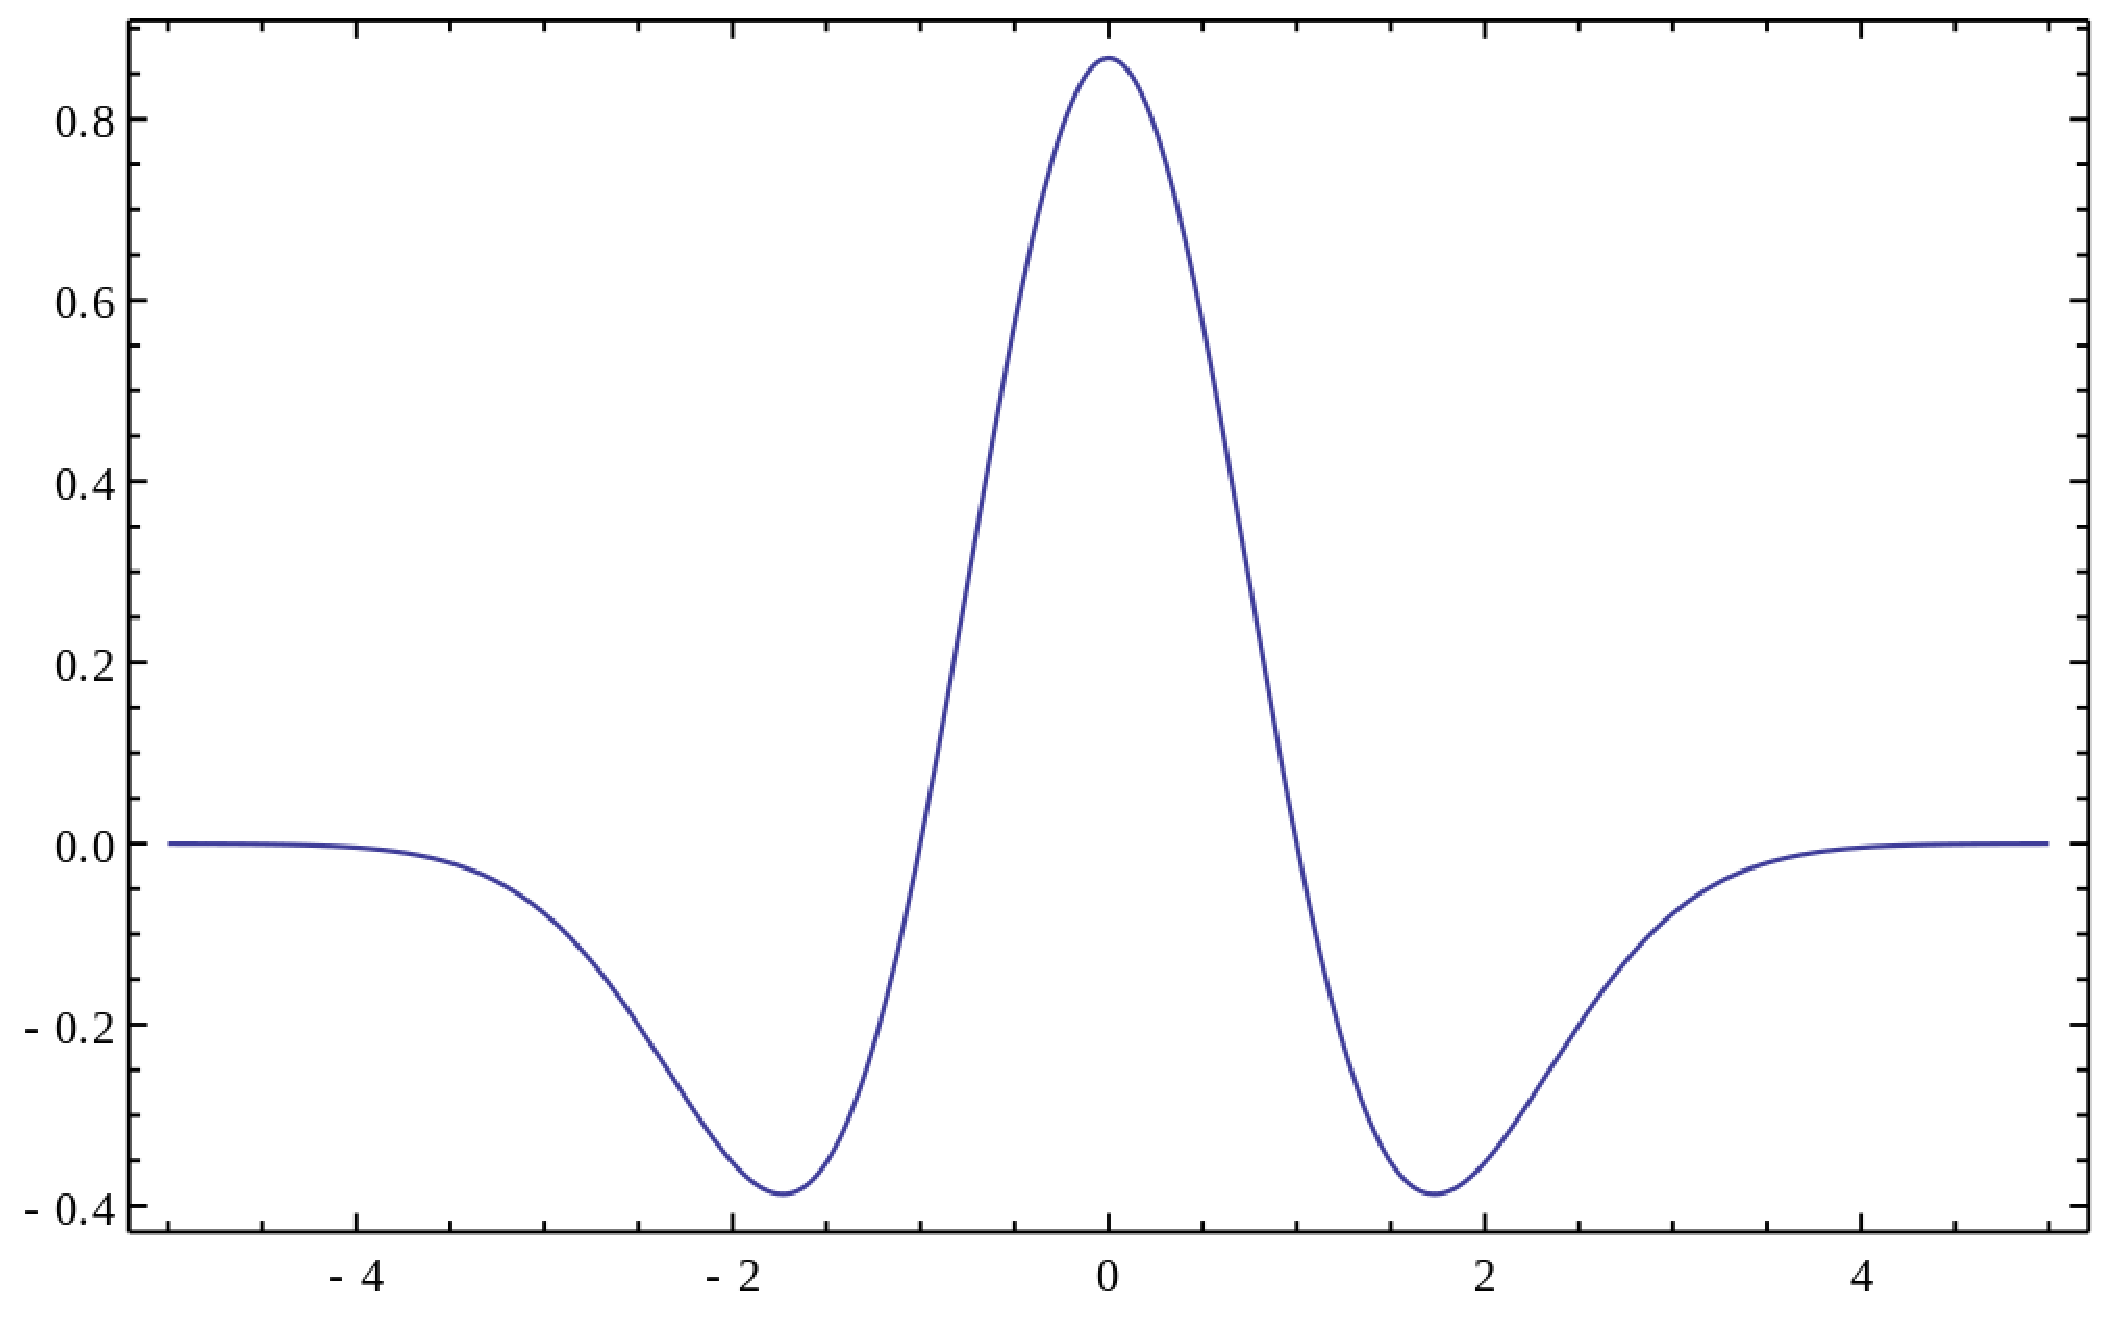
\includegraphics[width=.8\linewidth]{figure2}
  \caption{\label{fig:firstExample}
           Mexican Hat Wavelet.}
\end{figure}

In \cite{PG2011short:67-72:2011}, the computation of
wavelet-transformed velocity is only for particles in one size.  But in
our work, we have particles in two scales. The equation to compute
wavelet-transformed velocity in this paper is the same as that in
\cite{PG2011short:67-72:2011}. We use different scale $s$ for
particles in different size, and $s$ is usually the same as the kernel
length $h$. After generating the transformed velocity, we compute the
energy in frequency domain with: $$\hat{e}_i=\frac{1}{2}m_i\hat{u}_i^2
\quad \quad \quad \quad \quad \quad \quad \quad \quad \quad \quad
\quad(11).$$

\begin{figure}[htb]
  \centering
  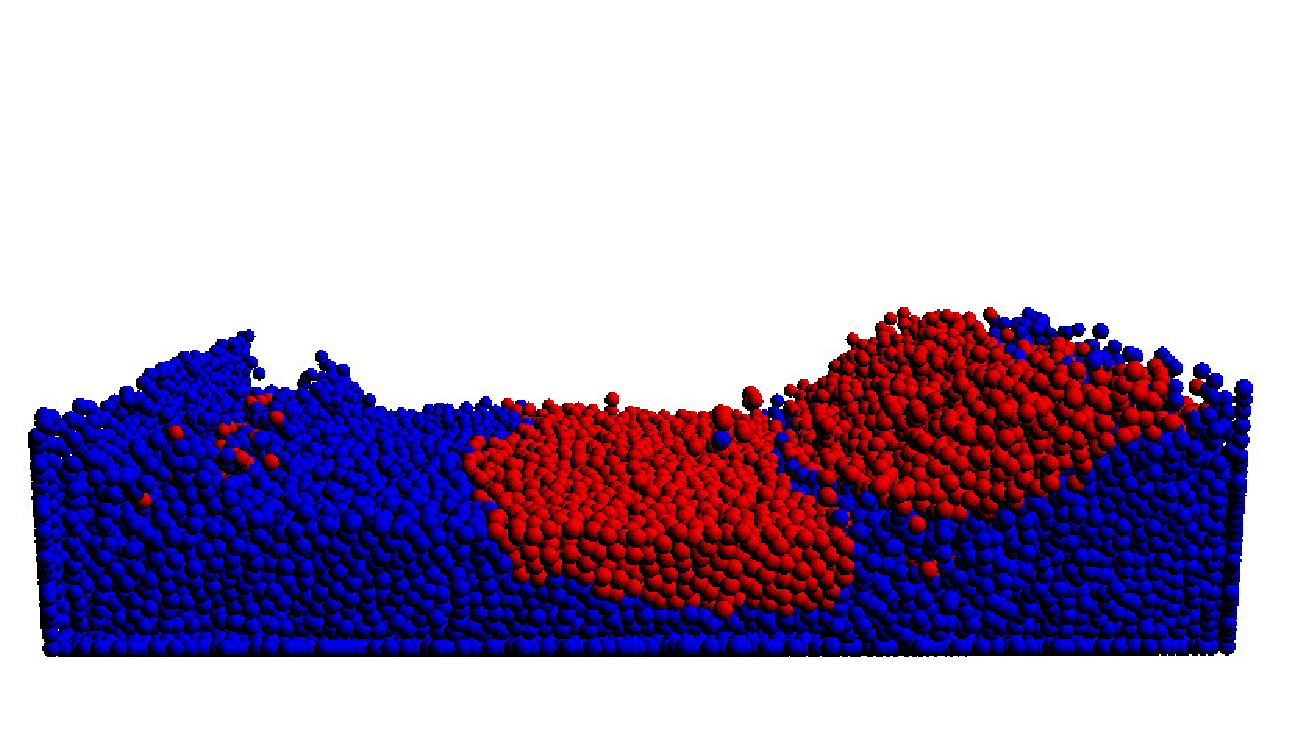
\includegraphics[width=.4\linewidth]{energy-1}
  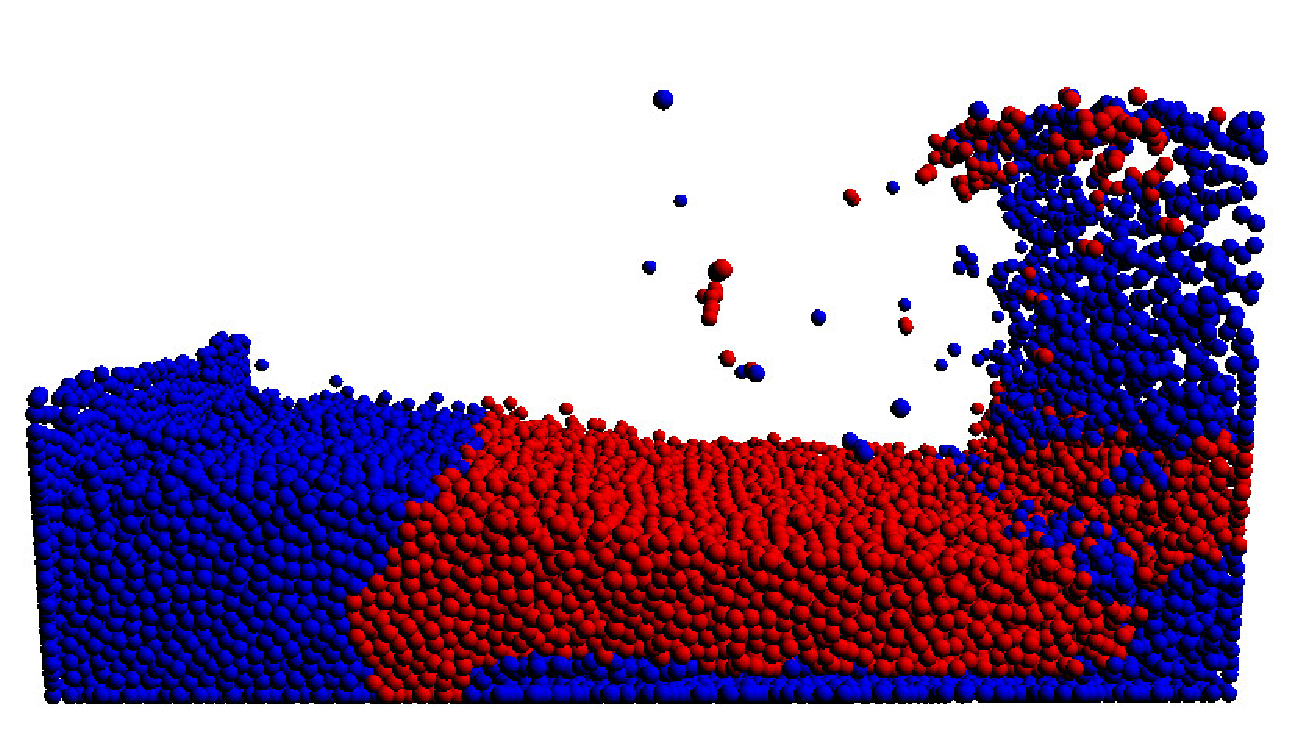
\includegraphics[width=.4\linewidth]{energy-2}
  \caption{\label{fig:firstExample}
           Energy distribution in 3D.}
\end{figure}

Figure 3 is the energy distribution generated with the equation
$(11)$. The red particle indicates the high energy level and blue one indicates
the low energy level.  The wavelet-transformed energy in frequency domain
could indicate the turbulent region.

%-------------------------------------------------------------------------
\subsection{Geometrically based Distance Value}

Geometry is another factor indicating where fluid details actually
exist. The visual importance of region always increases while it moves
approaching the fluid surface. Therefore, one naive way is that
we could split particles
near fluid surface and merge particles deep inside fluid. To find
all surface particles, we first find the fluid surface. We define
the fluid surface as an implicit function:
$$\phi(x)=|x-p|-h,  (12)$$

\noindent where $x$ is the sampled position, $p$ is the nearest
particle to position $x$ and $h$ is the kernel length of particle $p$.
$\phi > 0$ represents the air region and $\phi < 0$ represents the
fluid region. $\phi = 0$ is the fluid surface.

\begin{figure}[htb]
  \centering
  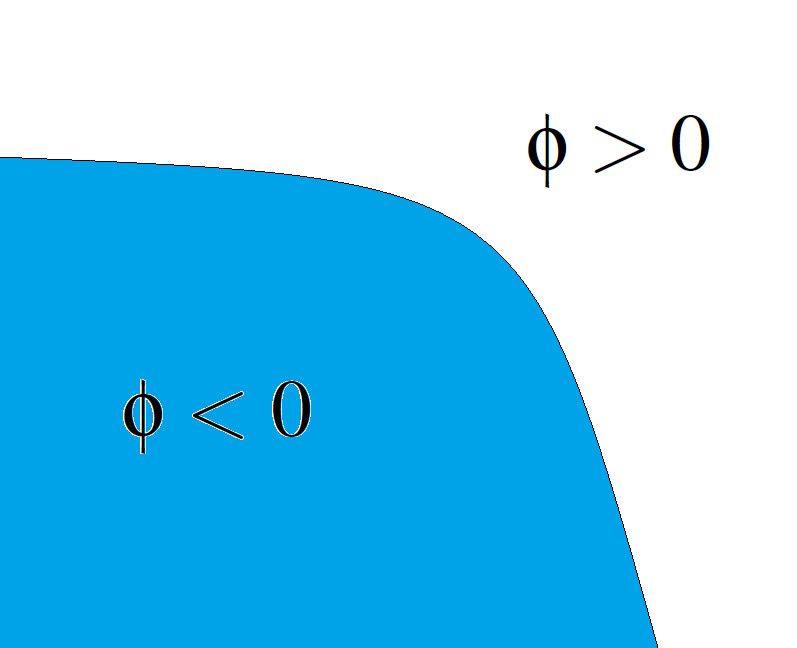
\includegraphics[width=.5\linewidth]{implicit}
  \caption{\label{fig:firstExample}
  Representation of surface with implicit function.
$\phi < 0$ is the fluid region and $\phi > 0$ is the air region.}
\end{figure}

We define all particles near fluid surface $\phi = 0$ as surface
particles. Unlike \cite{Adams:2007:ASP:1276377.1276437} which
accurately generated the distance
field for particles, we only approximate distance field in our algorithms.
In \cite{Adams:2007:ASP:1276377.1276437}, only one particle's distance
value would be computed for each iteration. In our method, we compute
distance values for a number of particles in each iteration.
For 20k particles, seven iterations are usually enough
as in Algorithm 1. Figure 5 is the example demonstrating the
approximate distance field of particles. Red particles are surface
particles. The darker the blue particle is, the closer
it is to the fluid surface.

\begin{figure}[htb]
  \centering
  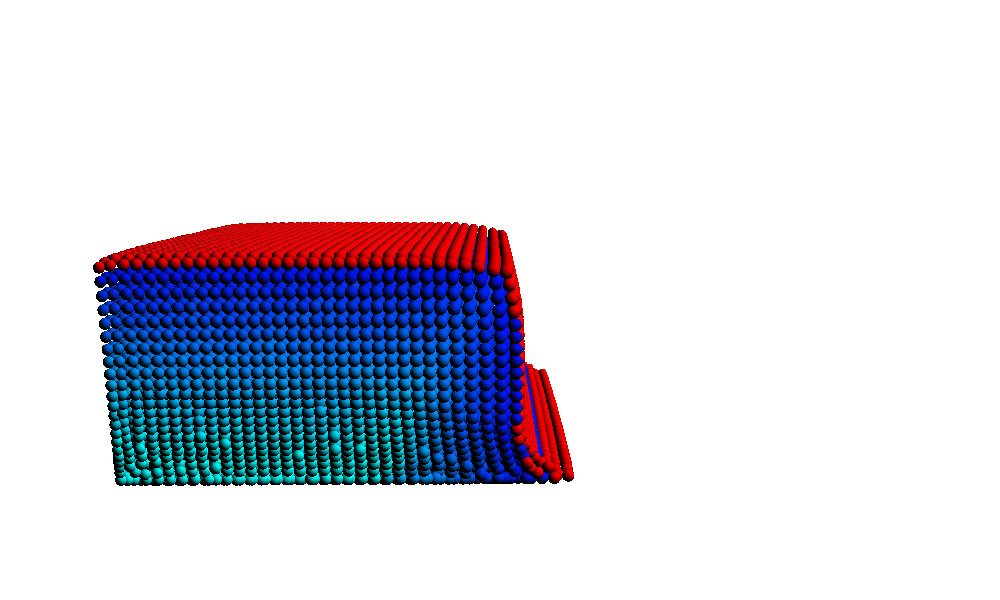
\includegraphics[width=.4\linewidth]{dist-1}
  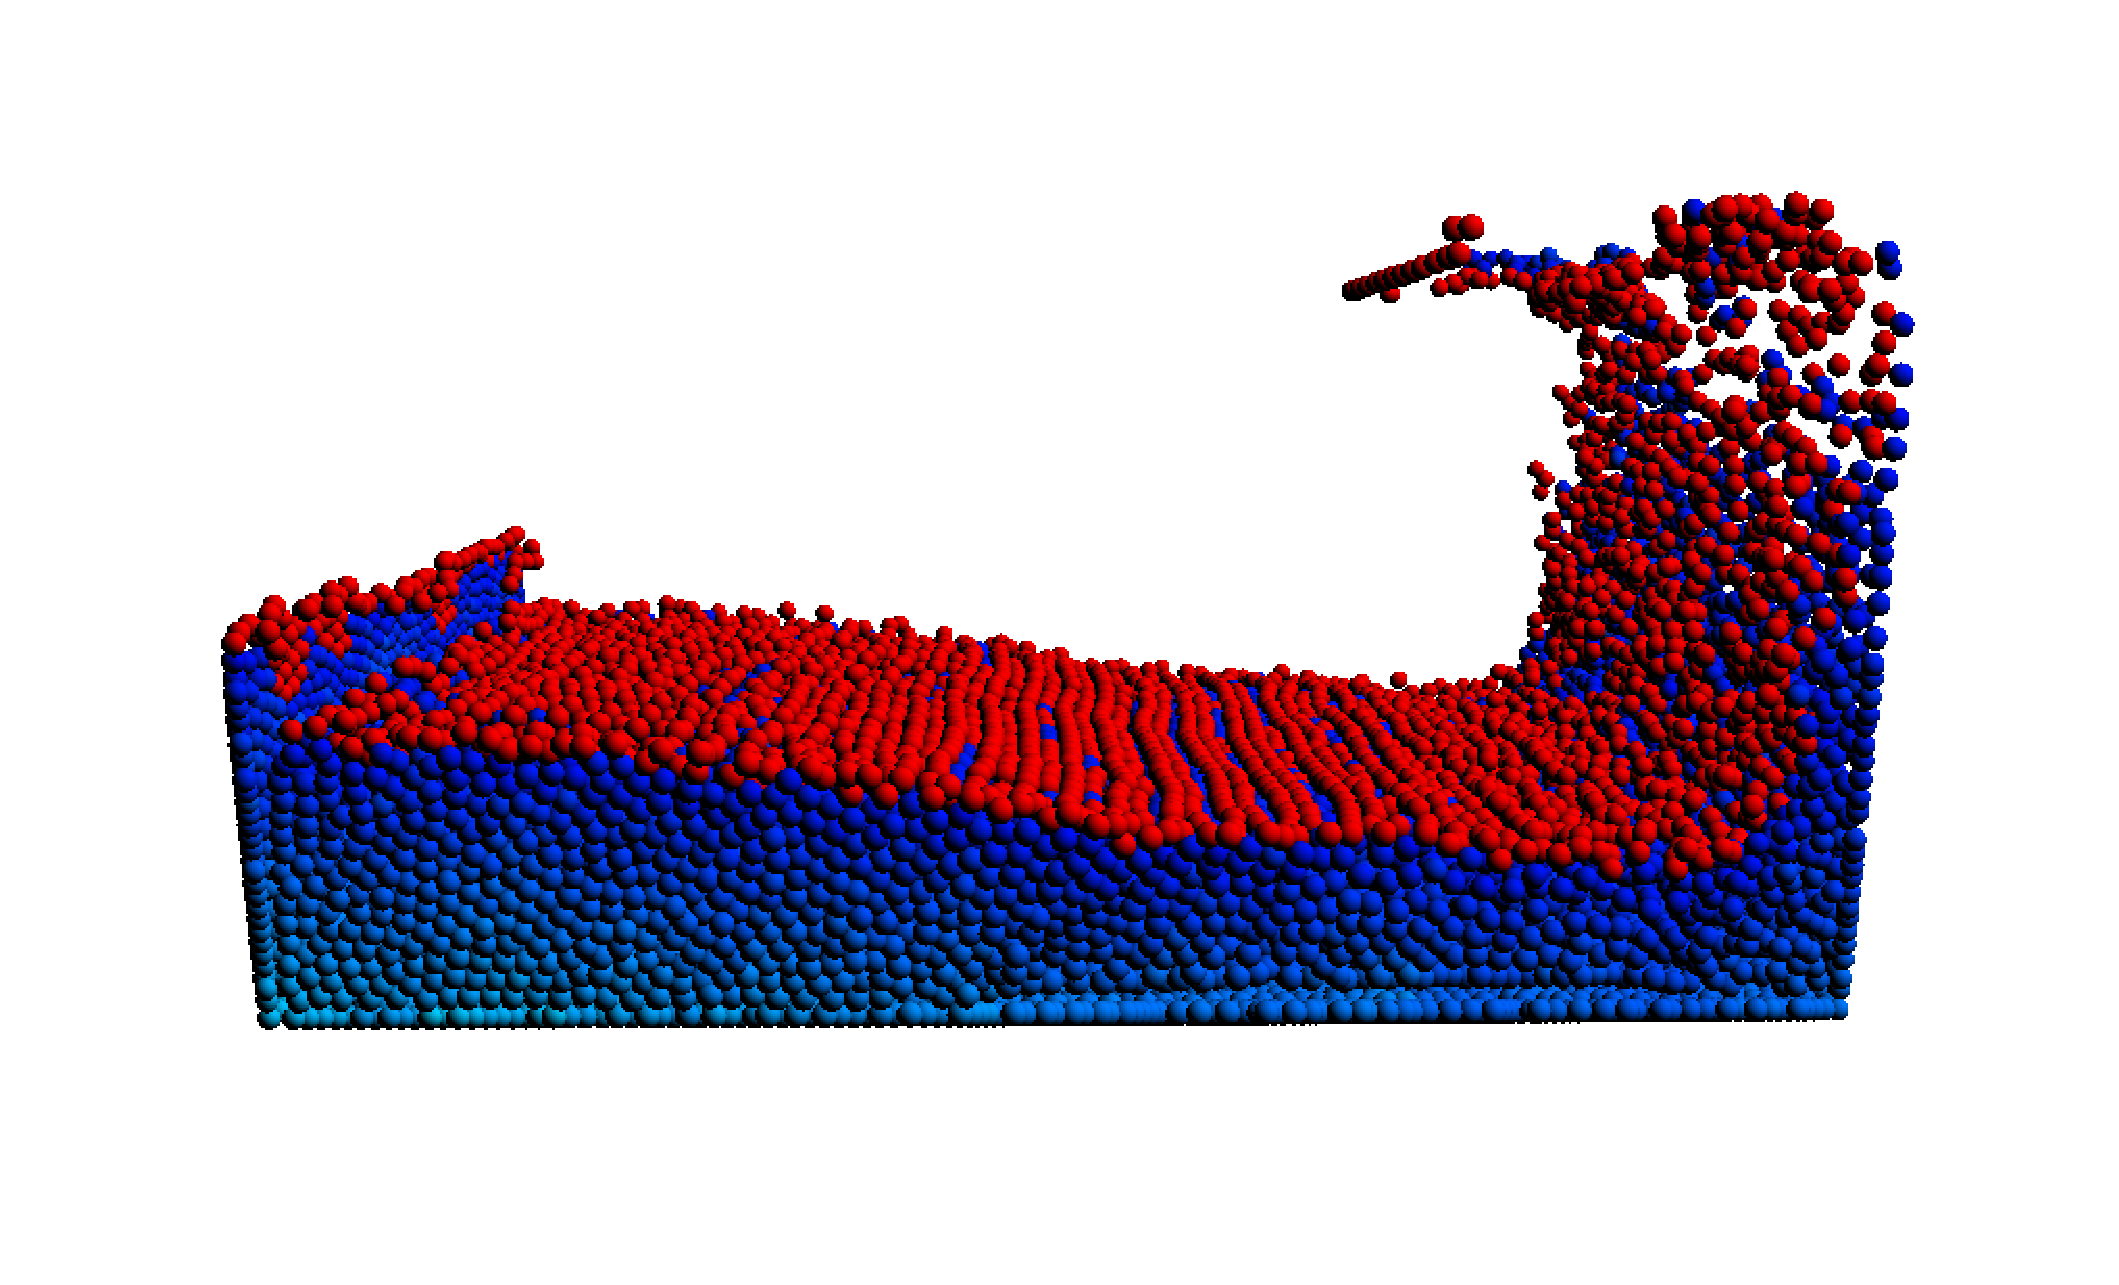
\includegraphics[width=.4\linewidth]{dist-2}
  \caption{\label{fig:firstExample}
           Distance field in 3D.}
\end{figure}

\begin{algorithm}[htb]
\caption{ Distance Field Approximation. }
\begin{algorithmic}[1]
\STATE Set the tag for each particle as $0$.
\STATE Set the tag for each surface particle as $1$. Set their distance value as $0$.
\STATE For all particles whose tag is $1$, propagate the distance value to their neighbors within kernel length $h$ (in one iteration).
\STATE If tags for all particles are $1$, Stop. Otherwise, go to Step $3$.
\end{algorithmic}
\end{algorithm}

%-------------------------------------------------------------------------
\subsection{Two Scale SPH Equation}

Since we are able to detect both high energy particles and particles
close to fluid surface, we could establish our criterion to guide
particle splitting and merging. Since our algorithm is both physically
and geometrically based, we define two sets of thresholds for both
physics and geometry. We denote that, $dist \_ merge$ and
$dist \_ split$ are two geometry thresholds, and
$energy \_ merge$ and $energy \_ split$ are two physical thresholds.

For a particle, if the energy $\hat{u} > energy \_ split$ \textbf{or}
distance field $d < dist \_ split$, we split the large particle into
small particles.
If the energy $\hat{u} < energy \_ merge$ \textbf{and} distance field $d > dist \_ merge$, we merge small particles into one large particle. We couple physics and geometry together.

We use the same equation in \cite{Muller:2003:PFS:846276.846298}
to compute the density for the particle. However, we
modify the constant gas equation as follows to guarantee
the incompressibility of fluid:
$$\rho=\kappa((\frac{\rho}{\rho_0})^7-1) \quad \quad \quad \quad \quad \quad\quad \quad \quad \quad(13)$$

Since two particles in different scales have different kernel length and
mass, unlike \cite{Adams:2007:ASP:1276377.1276437} we design a new
set of equations for particle pressure and viscosity computation:
$$F^{Pres}_i=-\sum_{j}\frac{m_j+m_i}{2}(\frac{p_i}{\rho_i^2}+\frac{p_j}{\rho_j^2})(\frac{\nabla W(x_{ij}, h_i)+\nabla W(x_{ij}, h_j)}{2}) (14),$$
and
$$F^{Visc}_i=\mu\sum_{j}\frac{V_i+V_j}{2}(v_j-v_i)\frac{\nabla^2W(x_ij, h_i)+\nabla^2W(x_ij, h_j)}{2} (15),$$

\noindent with $V=\frac{m}{\rho}$ the particle volume.

%-------------------------------------------------------------------------
\subsection{Merging and Splitting}

We use a similar method as in \cite{Hong:2008:API:1394332.1394340}
to merge and split particles.
When merging a group of particles, the new particle is placed at the center of
gravity of all original particles. We can compute the mass, kernel length,
position and velocity of the newly created particle $i$ from
all particle members forming the new particle $j$ by:
$$m_i=\sum_{j} m_j \quad \quad h_i=\sqrt[3]{\sum_{j}h_j^3}$$
$$x_i=\frac{\sum_{j}x_j V_j}{\sum_{j}V_j} \quad \quad u_i=\frac{\sum_{j}u_j V_j}{\sum_{j}V_j}$$

\noindent where $h$ is the particle kernel length.

Unlike merging, the splitting of a large particle is performed by creating
a new set of $n$ particles. In our video demonstration, we set $n$ as $3$.
With a larger $n$ we could generate better visual effects. The mass, kernel
length and velocity of each new particle are computed by the following
equations:
$$m_j=\frac{m_i}{n} \quad \quad  h_j=\sqrt[3]{\frac{h_i^3}{n}} \quad \quad u_j=u_i$$

There are multiple ways to determine the position of the new generated sub
particles. We choose to place them randomly at the position within the radius
of the original large particle. For more details on particle splitting and
 merging, please refer to \cite{Hong:2008:API:1394332.1394340}.

We summarize the algorithm in Algorithm 2.

\begin{algorithm}[htb]
\caption{Wavelet based Adaptive SPH.}
\begin{algorithmic}[1]
\STATE Find the fluid surface according to the implicit function.
\STATE Generate the distance field for particle system.
\STATE Compute particle wavelet energy.
\STATE Compute density and pressure for each particle.
\STATE Compute the velocity of particle.
\STATE Split and merge the particle.
\STATE Reconcile the velocity of particle based on air resistance.
\STATE Advect the particle to the new position.
\end{algorithmic}
\end{algorithm}

%%%
%%% Note to Dongli:
%%% Hong is currently here, finishing the editing till the start of
%%% Section: Surface Tension here
%%% Continue continue next
%%%


%-------------------------------------------------------------------------
\section{Surface Tension}

We also design a new surface tension model. In previous work
\cite{Muller:2003:PFS:846276.846298}, the surface tension is only
based on the interaction between surface particles. The concept of
color field\cite{Muller:2003:PFS:846276.846298} has been proposed
before. The surface tension is derived from both gradient and
Laplacian of gradient field. Surface particles are always particles
whose normalization of gradient of color field is larger than the
pre-defined threshold value. In our work, we regard particles near
implicit function as surface particles. But we use the same method to
compute surface tension for surface particles. To make the simulation
more physically accurate, we integrate the air resistance into
simulation.

In \cite{Schechter:2012:GSA:2185520.2185557}, people apply ghost air
particles to integrate the surrounding air into simulation. By
generating a set of ghost air particles near the fluid surface, we
could have air participating into simulation. However,
\cite{Schechter:2012:GSA:2185520.2185557} requires the sampling of air
particles near the fluid surface, which is a complex process. To
balance the simulation performance of physical accuracy, we substitute
the ghost air particles with air resistance force. We consider this
force from the pure geometry's perspective instead.

We first find the surface normal vector $\vec{d}$ from surface
particle pointing outside to air region according the gradient of
color field. Then we project the velocity of particle $\vec{v}$ onto
the surface normal vector $\vec{d}$. The result length $l$ is the
result of dot product$\vec{d} \cdot \vec{v}$. If $l$ is larger than
$0$, the particle is moving outward the fluid. Then we need to apply
the air resistance force on the particle with the following equation:
$AirForce=-(\vec{d} \cdot \vec{v})\times c$, where $c$ is a user
defined coefficient to control the air resistance magnitude.

\begin{figure}[htb]
  \centering
  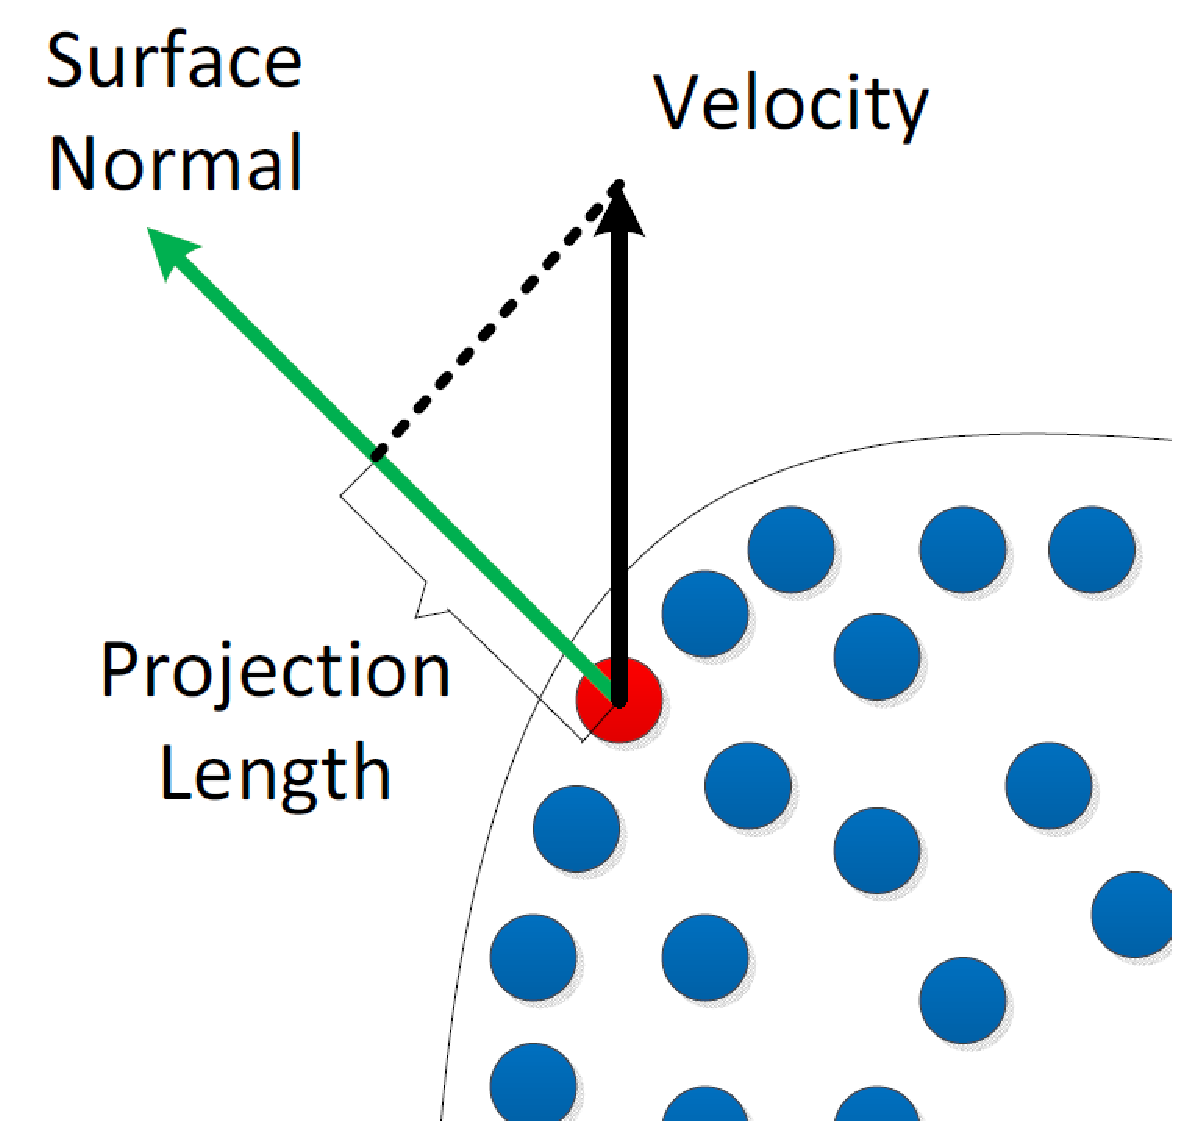
\includegraphics[width=.6\linewidth]{surface}
  \caption{\label{fig:firstExample} Our surface model. Red particle is
    the surface particle moving outward. Green arrow is the surface
    normal and black arrow is the velocity of particle.}
\end{figure}

In Figure 6, the red particle is moving outward the fluid. Green arrow
is the surface normal generated from the gradient of color field and
the black arrow is the current velocity of particle.  We project the
black arrow onto the green arrow to compute the resistance magnitude
from air. The algorithmic details are documented in Algorithm 3.

\begin{algorithm}[htb]
\caption{Surface Tension}
\begin{algorithmic}[1]
\STATE Apply surface tension as in \cite{Muller:2003:PFS:846276.846298} to all surface particles.
\STATE Compute the gradient vector from surface particle to air (based on gradient of color field).
\STATE Project the velocity of particle onto its surface normal vector, and compute the length $l$.
\STATE $AirForce=-(\vec{d} \cdot \vec{v})\times c$, $c$ is a user defined coefficient to control the air resistance magnitude.
\end{algorithmic}
\end{algorithm}

%%%
%%% Dongli, I did NOT touch the entire section of Implementation and Results
%%%
%%% But I changed the title of this section!!!
%%%
%%%
%%%

%-------------------------------------------------------------------------
\section{Implementation and Experimental Results}

We have implemented our SPH simulator with C++. All examples in this paper are implemented on a 64-bit machine with four 2.40 GHZ Core i7 CPU and 8GB memory.
After extrapolating the surface triangular mesh with marching cube, we render the fluid with POV-Ray.

In Figure 7, we demonstrate with animation in our method. Pictures on the left side are simulation directly rendered as particles.
Picture of the right side are corresponding fluid rendered with POV-Ray. Simulation begins with about 220k small size particles. Merging and splitting
are dynamically happen during the simulation. Yellow particles are small size particles and red particles are large size particles. Each large particle
is equivalent to three small particles. According to the demonstration, our method could detect the turbulent region and refine the simulation effectively.
In Figure 7(c), fluid on top layer is moving toward left side. Because the left side is turbulent, we refine the simulation in region even deep inside fluid on left side.
Table 1 is the set of parameters of simulation.

Table 2 is the experiment result. One purpose in adaptive SPH is to improve the performance of simulation. Because our algorithm is not implemented on GPU,
it would take more time for each frame compared to the traditional SPH algorithm. However, according to the experiment results in Table 2, the bottleneck of
performance is surface tracking. $60\%$ of simulation costs are for surface tracking, which is used to find all surface particles.
 We find all surface particles with the fast marching algorithm with an auxiliary grid of resolution $128 \times 64 \times 64$. The
performance of fast marching algorithm on CPU is $O(N)$. Since this could be ported to GPU, the performance would be constance $O(1)$ time. And the bottleneck for performance could be
avoided.

~\\
~\\
\begin{center}
    \begin{tabular}{ | l | l | l |}
    \hline
    \multicolumn{3}{|c|}{Simulation Parameters} \\
    \hline
    Parameter & Value & Unit \\ \hline
    Large Kernel & $0.04$ & $m$ \\ \hline
    Large Mass & $0.02$ & $kg$ \\ \hline
    Gravity & $3.2$ & $m/s$ \\ \hline
    Rest density  & $1000$ & $kg/m^3$ \\ \hline
    Gas Constant  & $1.0$ & $N/A$ \\ \hline
    Viscosity  & $10.5$ & $Pa \cdot s$ \\ \hline
    Time Step & $0.001$ & $s$ \\ \hline
    \end{tabular}

    \textbf{Table 1}. Simulation Parameters
\end{center}

%%%
%%%
%%% Note to Dongli:
%%% I did not modify your implementation and experimental results section
%%% But I have changed the section title
%%%
%%% I have also modified the conclusion section!!!

%-------------------------------------------------------------------------
\section{Conclusion and Future Work}

We have developed a novel technique for particle based fluid
simulation that takes advantage of our new refinement and
simplification mechanism. Such mechanism is founded up the hybrid of
physics and geometry. In particular, we use both the
wavelet-transformed energy and distance field to guide the particle
splitting and merging. With our adaptive SPH algorithm, not only
regions near fluid surface but also highly turbulent regions anywhere
within fluid can be properly handled whenever and wherever particle
splitting and merging are necessary. Consequently, high-fidelity SPH
simulation supporting dramatic turbulence and small-scale details can
be achieved effectively. The detection and refinement of microscopic
material interface can also directly benefit from the utility of this
algorithm, as abrupt material change can be more accurately analyzed
in frequency domain. Through comprehensive experiments, we have
demonstrated that our method could preserve high quality visual
details. One limitation is that, the current animation system is not
yet parallel, as the implementation is entirely in CPU (not GPU). We
would like to upgrade our prototype system with CUDA which is our
ongoing research efforts.

%-------------------------------------------------------------------------

%\bibliographystyle{eg-alpha}
\bibliographystyle{eg-alpha-doi}

\bibliography{egbibsample}

%-------------------------------------------------------------------------
\newpage

\onecolumn
~\\
\begin{center}
   \begin{tabular}{l*{6}{c}r}
        Particles & Normal SPH Time & Adaptive SPH Time & Surface Tracking & Split-Merge \\
        \hline
        $16000$ & $107(ms)$ & $405(ms)$ & $248(ms)$ & $2(ms)$ \\
        $120k$ & $1508(ms)$ & $3123(ms)$ & $1869(ms)$ & $19(ms)$ \\
        $960k$ & $12.5(s)$ & $21.6(s)$ & $12.9(s)$ & $104(ms)$ \\
    \end{tabular}

    \textbf{Table 2}. Experiment Results
\end{center}

\begin{figure*}[tcb]
  \centering
    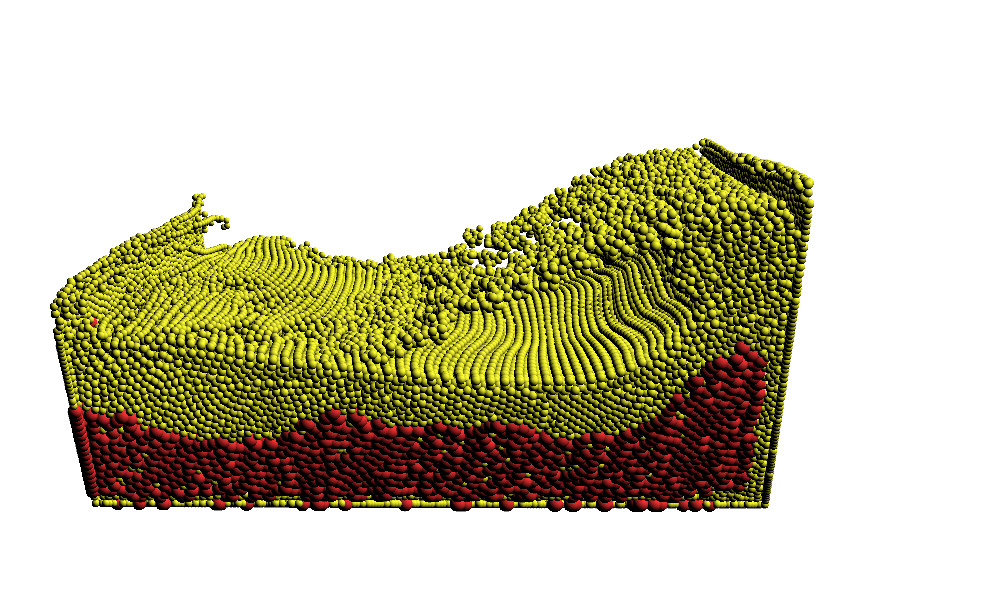
\includegraphics[width=.4\linewidth]{demo-2} \quad \quad
    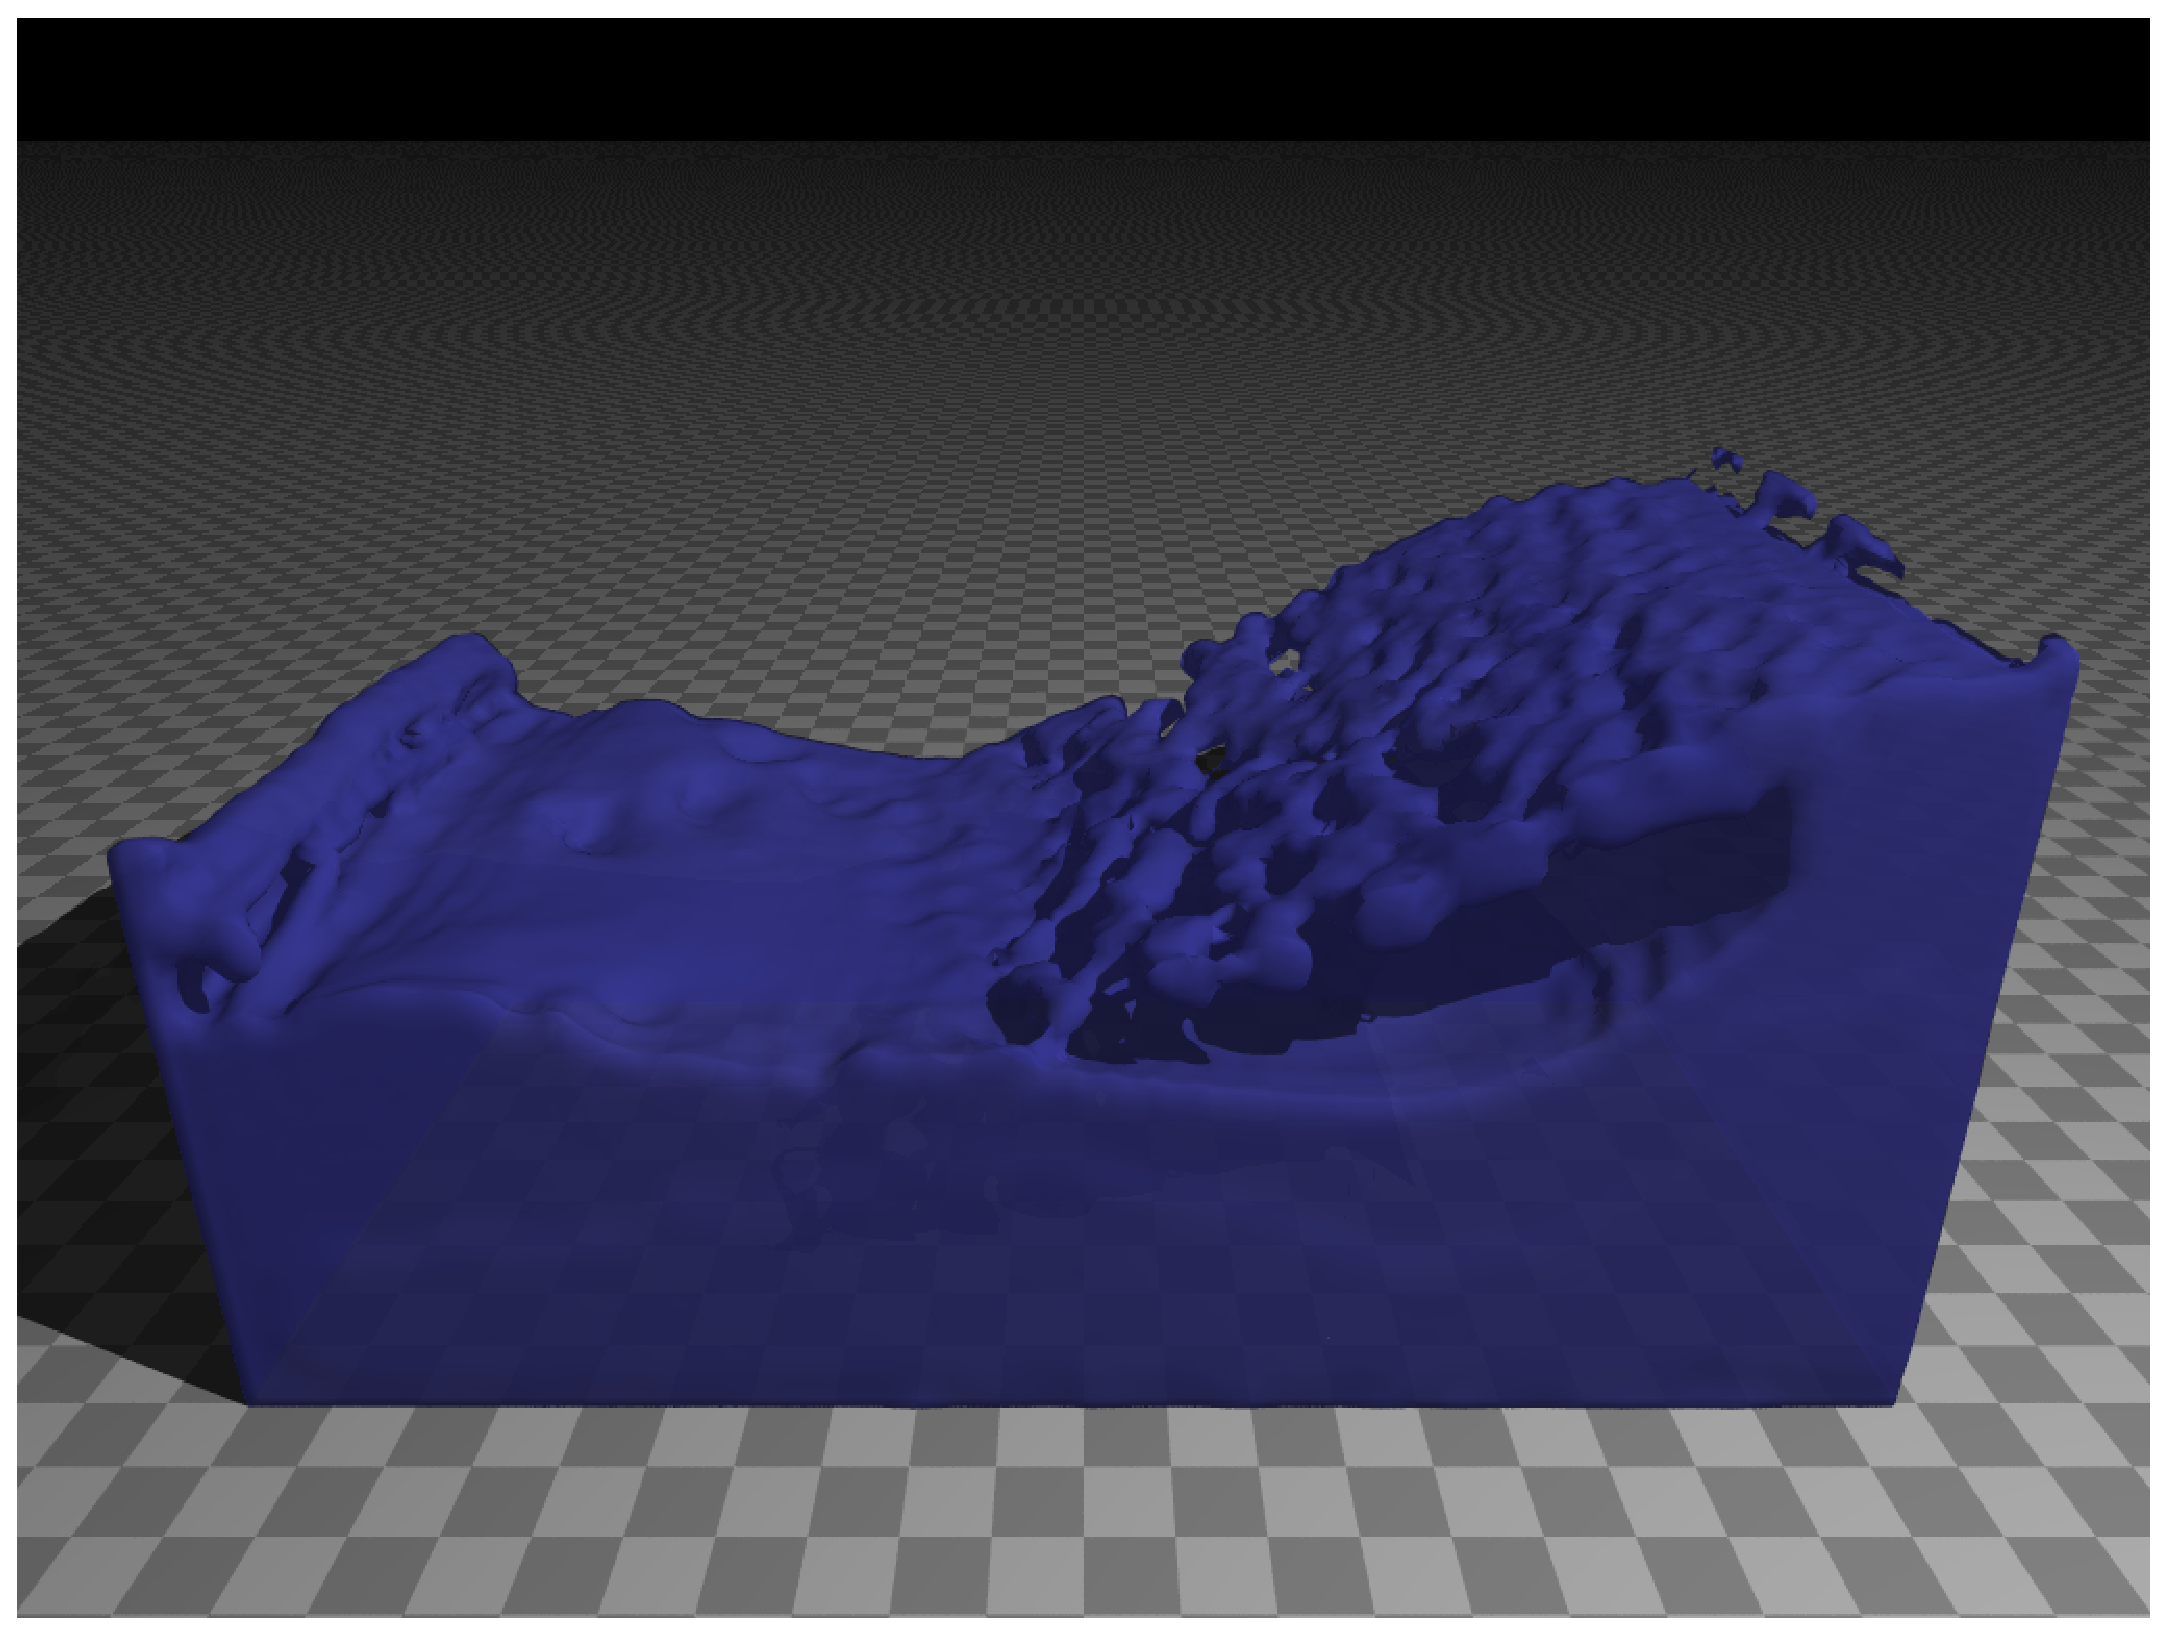
\includegraphics[width=.4\linewidth]{demo-1}

    \textbf{Figure 7(a)}

    \hfill

    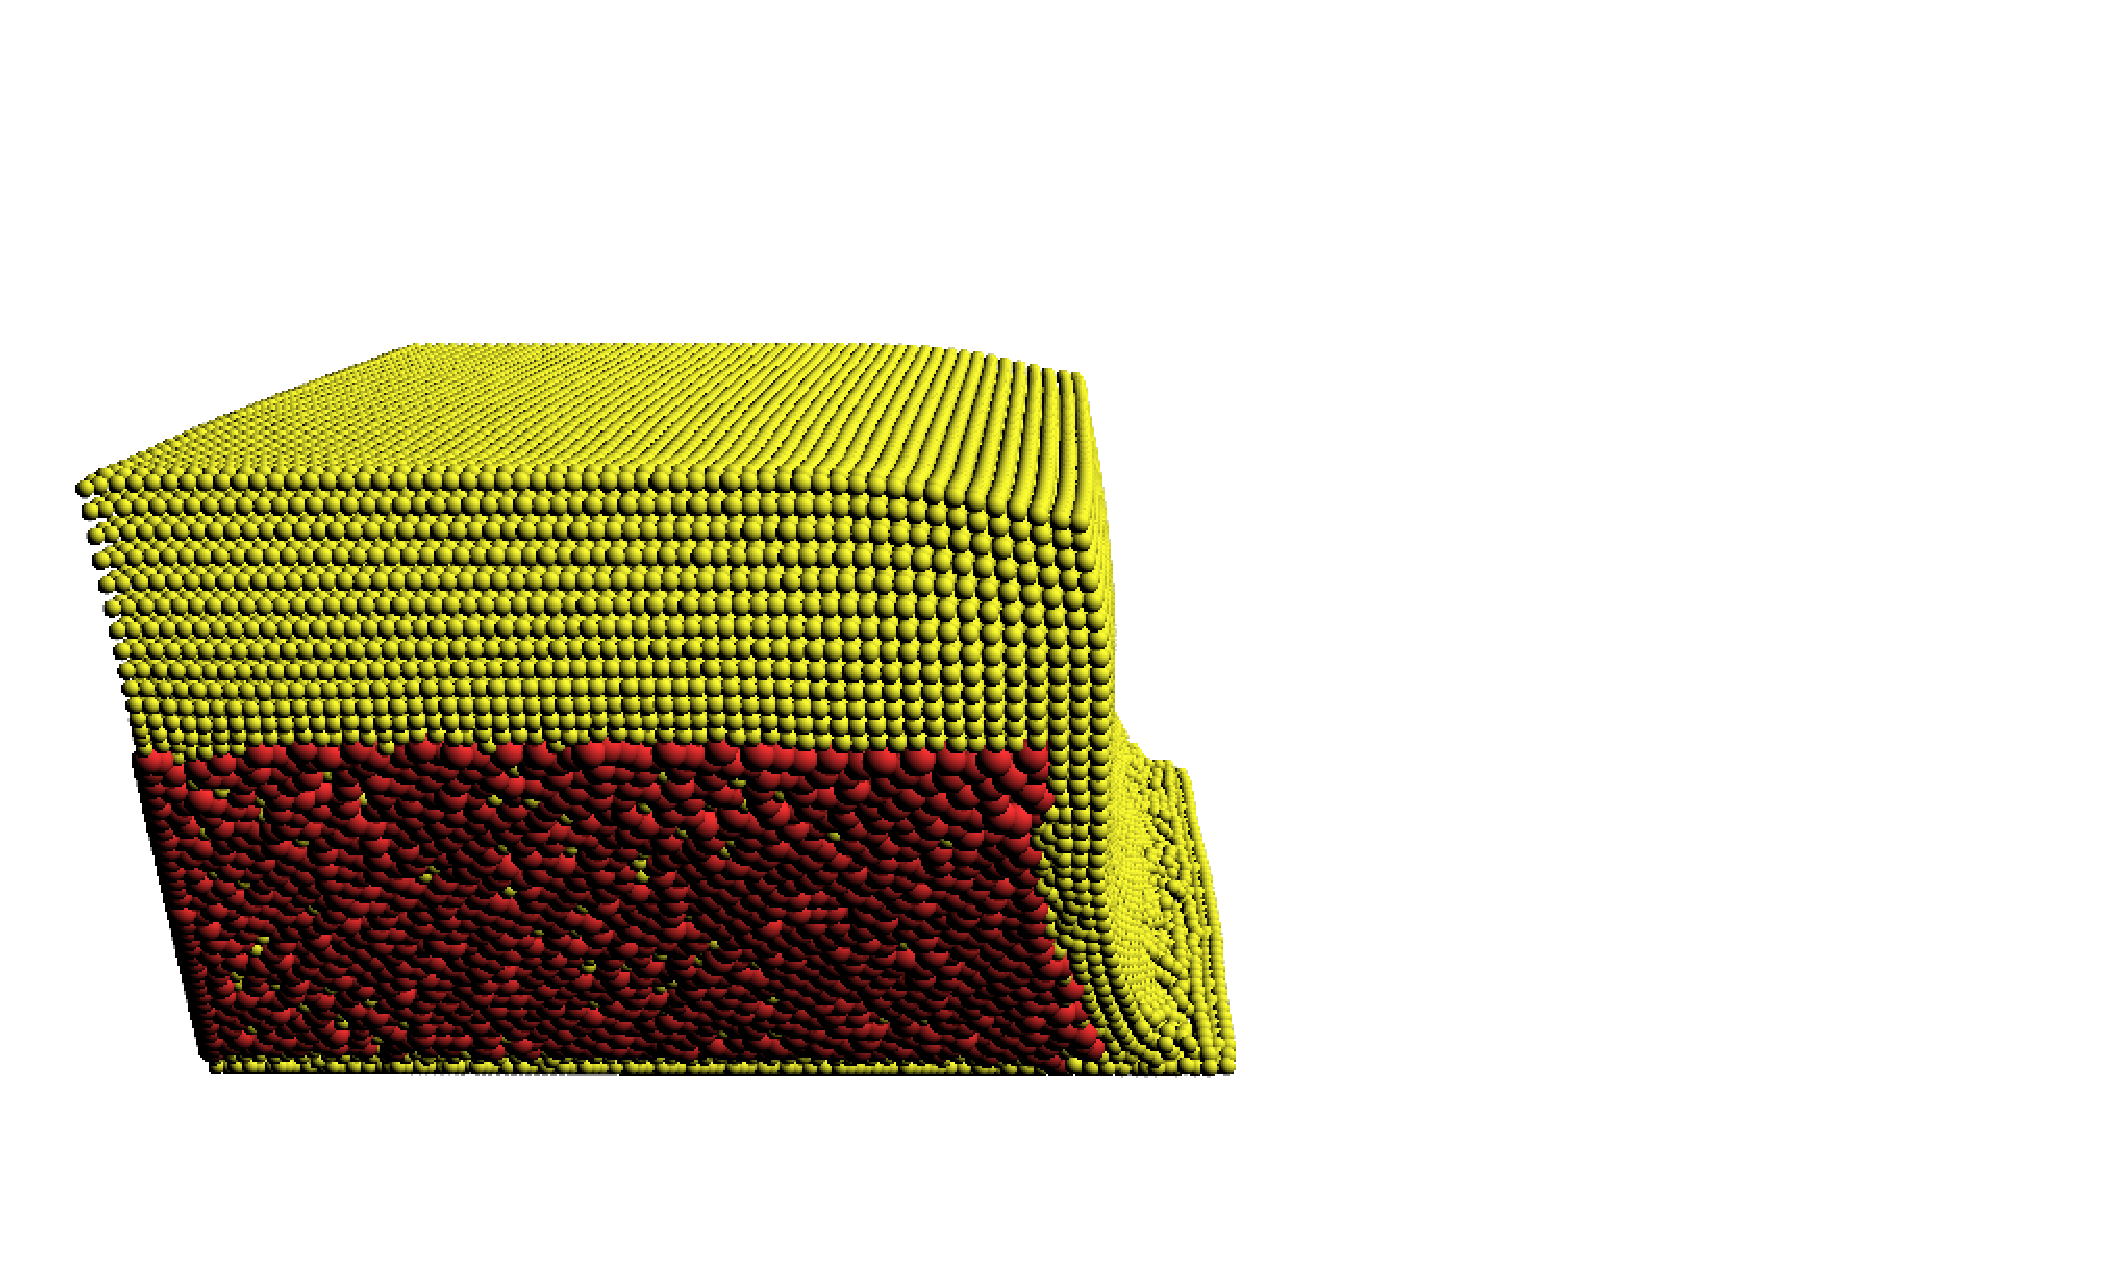
\includegraphics[width=.4\linewidth]{demo-4} \quad \quad
    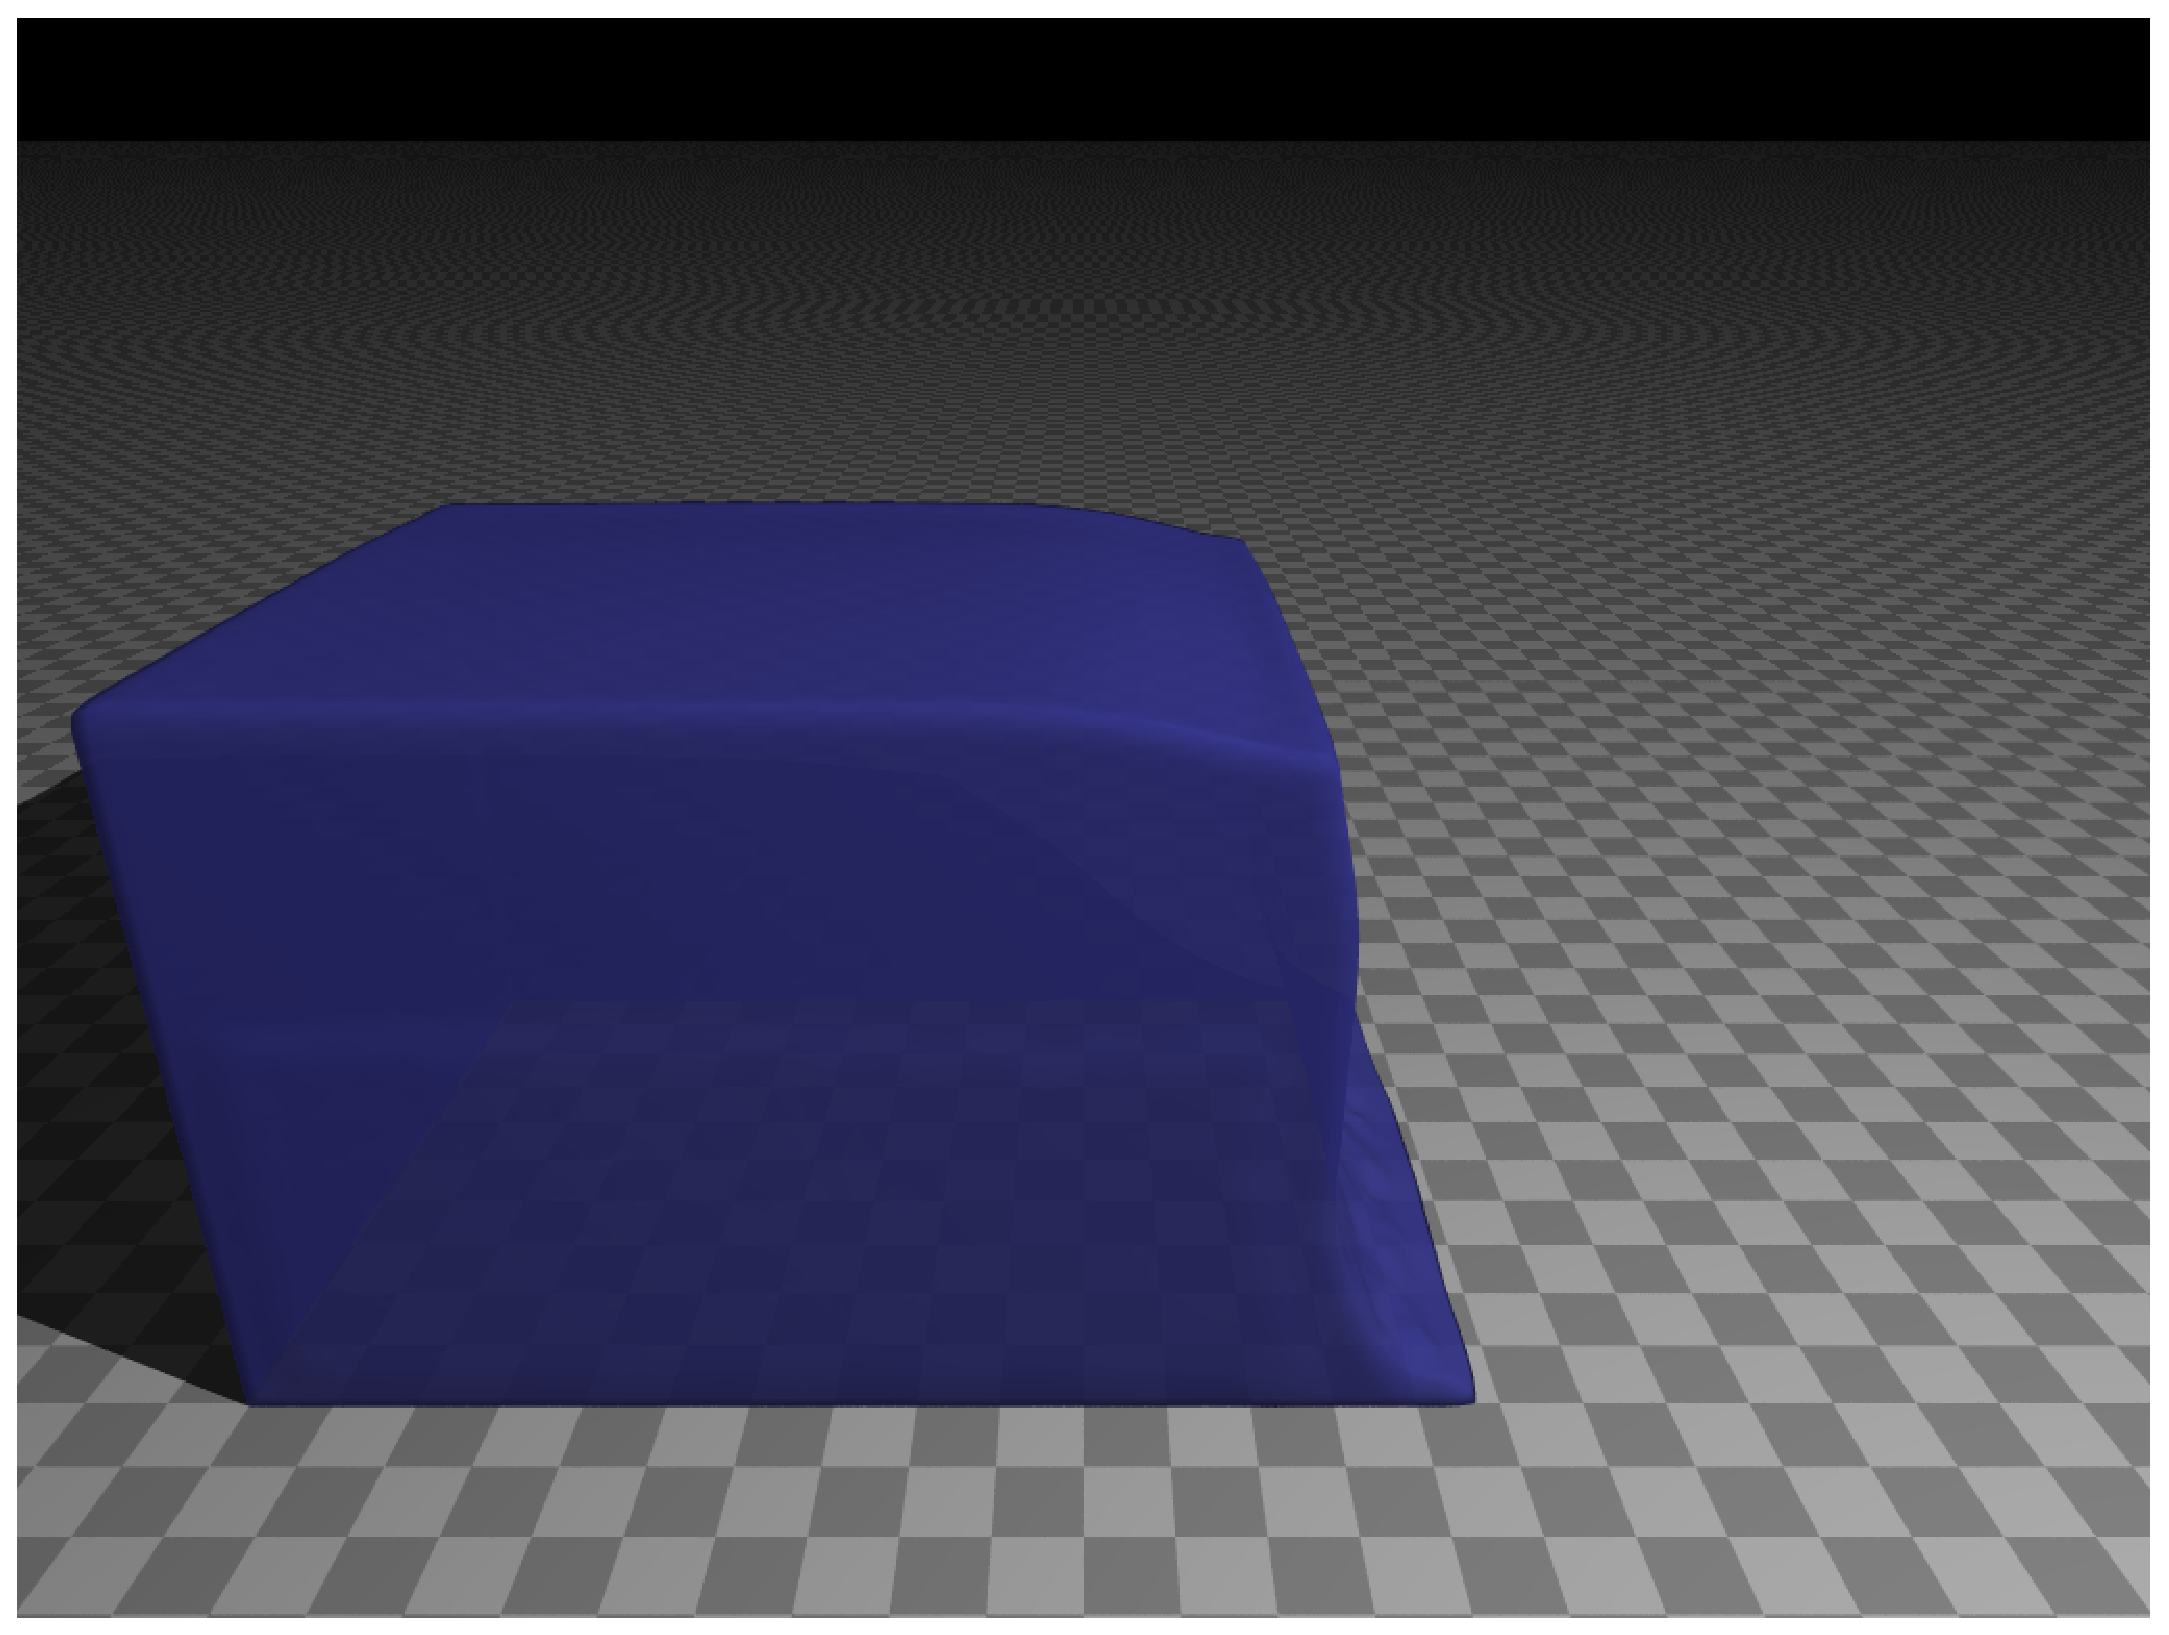
\includegraphics[width=.4\linewidth]{demo-3}

    \textbf{Figure 7(b)}

    \hfill

    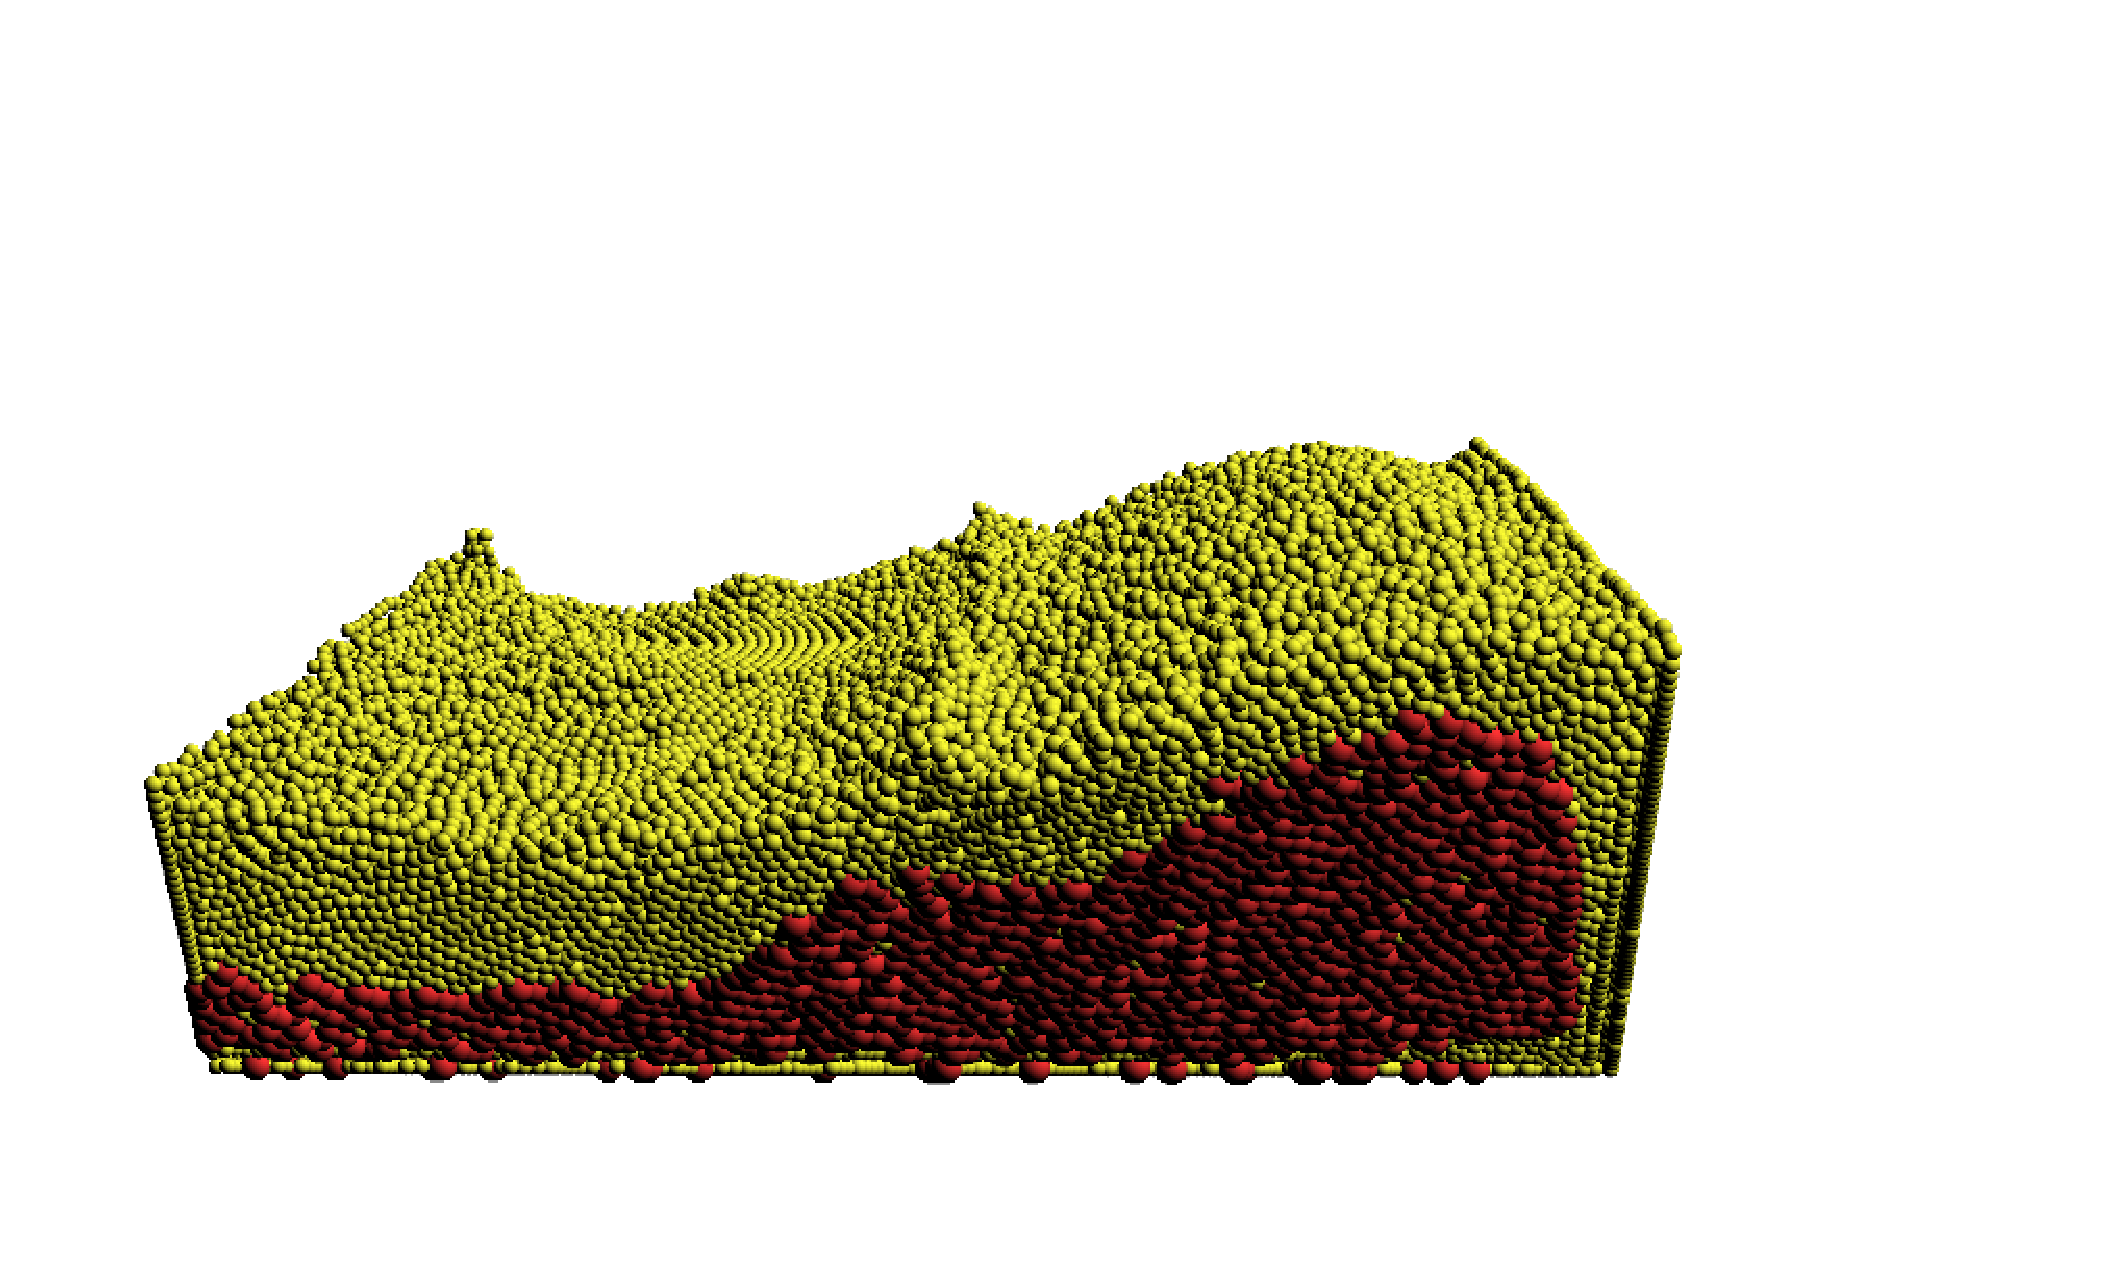
\includegraphics[width=.4\linewidth]{demo-6} \quad \quad
    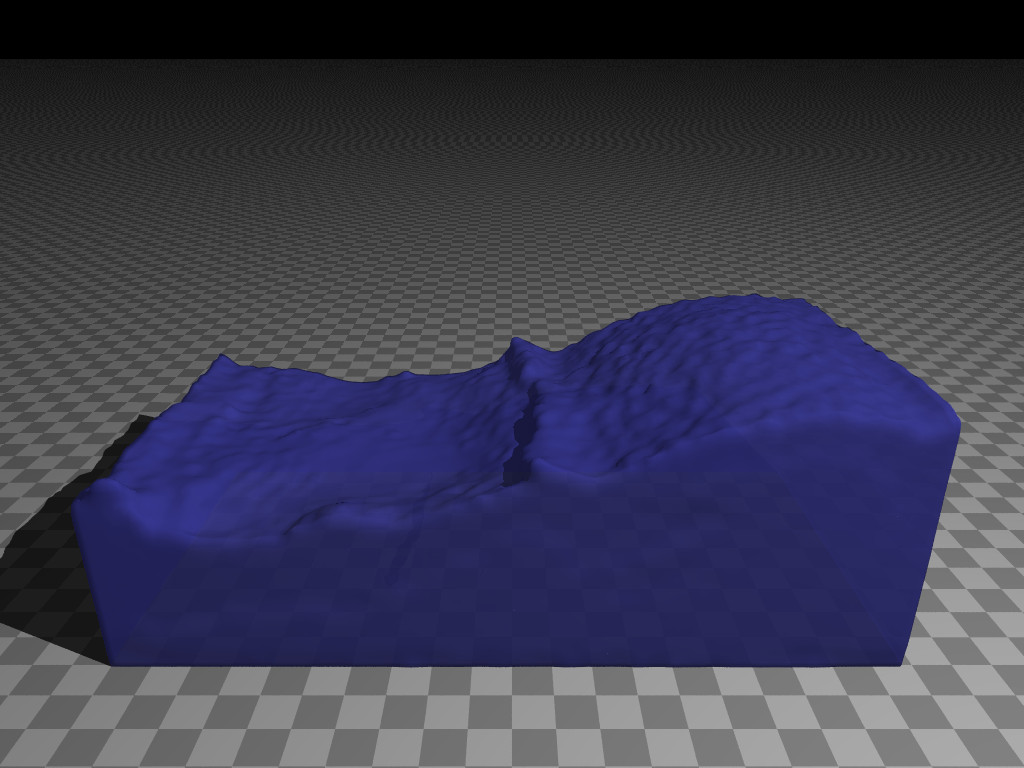
\includegraphics[width=.4\linewidth]{demo-5}

    \textbf{Figure 7(c)}
  \caption{The example showing the hybrid approach with 220k particles.}
\end{figure*}

\end{document}
